%****************************************************
%	CHAPTER 7 - RESULTS
%****************************************************
\chapter{Results}
\label{ch:results}
%====================================================
\section{Sensor Characterisation}
\label{sec:ch7.section1}
%----------------------------------------------------

%----------------------------------------------------
\subsection{Target Scene Reconstruction}
\label{subsec:ch7.section1.subsec1}

For each target, a single frame was inspected and the dimensions of the target were estimated where possible. This was achieved by visually identifying individual points that represented the extremities of the target in each axis, and measuring the distances between these points. The number of points in the frame, the overall accuracy of the target reconstruction and presence of undesirable artefacts such as shadowing and beam divergence effects were also noted. Subsequently, multiple frames were concatenated to create a denser point cloud of the target, and the dimensions were re-estimated. This process was repeated for a higher number of concatenated frames to observe the effect of increasing point density on the accuracy of the target reconstruction. The results for each target are detailed below. The target dimensions, as shown in Figure \ref{fig:target_dim}, were Height (H) = 180 mm, Length (L) = 1220 mm and Width (W) = 1130 mm. 

%----------------------------------------------------
\begin{figure}[H]
    \centering
    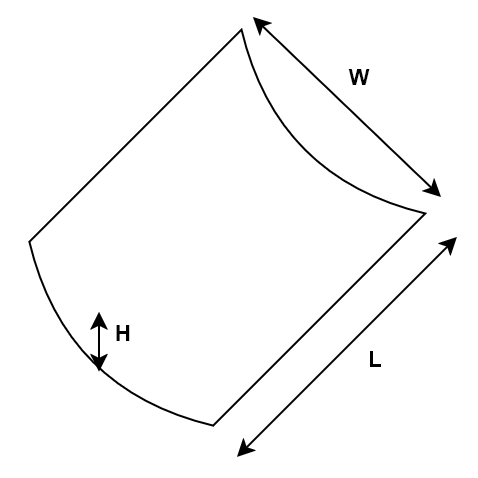
\includegraphics[width=0.4\textwidth]{figs/target_dim.png}
    \caption{\textbf{Target Dimensions.}}
    \label{fig:target_dim}
\end{figure}
%----------------------------------------------------

%----------------------------------------------------
\begin{table}[H]
\centering
\begin{tabular}{|l|r|r|c|r|}
\hline
\multicolumn{1}{|c|}{\textbf{No. Frames}} &
  \multicolumn{1}{c|}{\textbf{Height (mm)}} &
  \multicolumn{1}{c|}{\textbf{Length (mm)}} &
  \multicolumn{1}{c|}{\textbf{Width (mm)}} &
  \multicolumn{1}{c|}{\textbf{No. Points}} \\ \hline
1  & 150 & 1119 & NaN & 37  \\ \hline
4  & 153 & 1179 & NaN & 157 \\ \hline
10 & 153 & 1206 & NaN & 389 \\ \hline
\end{tabular}
\caption{Target A Reconstruction Dimensions}
\label{tab:target_a}
\end{table}
%----------------------------------------------------

In the single frame reconstruction, it was difficult to identify the curved shape of the target facing the sensor due to the low point density present. The high level of self-shadowing on the far side of the target also made it impossible to estimate the width of the target. As more frames were concatenated, the point density increased, allowing for a better identification of the curved shape facing the sensor and an improved length estimation. However, the width remained unmeasurable due to persistent shadowing effects. The estimated height of the target remained relatively consistent across all frame counts, with the length estimation improving with increased point density. Four concatenated frames allowed for the general geometry to be identified, while ten frames provided a moderate point density that marginally improved shape and dimension identification. In all cases, a combination of shadowing and bean divergence effects created a distortion on the far side of the target, resulting in a long 'tail' of points extending away from the target, as seen in Figure \ref{fig:A10Mesh}.

%----------------------------------------------------
\begin{table}[H]
\centering
\begin{tabular}{|l|c|c|c|r|}
\hline
\multicolumn{1}{|c|}{\textbf{No. Frames}} & \textbf{Height (mm)} & \textbf{Length (mm)} & \textbf{Width (mm)} & \multicolumn{1}{l|}{\textbf{No. Points}} \\ \hline
1  & NaN                      & NaN                       & NaN                       & 47  \\ \hline
8  & \multicolumn{1}{r|}{138} & \multicolumn{1}{r|}{1008} & NaN                       & 348 \\ \hline
15 & \multicolumn{1}{r|}{138} & \multicolumn{1}{r|}{1130} & \multicolumn{1}{r|}{1163} & 627 \\ \hline
\end{tabular}
\caption{Target B Reconstruction Dimensions}
\label{tab:target_b}
\end{table}
%----------------------------------------------------

Target B proved to be the most challenging to reconstruct due to its geometry, which featured a trough-like shape perpendicular to the sensor's line of sight that created significant self-shadowing effects. In the single frame reconstruction it was not possible to estimate any dimensions or identify the shape of the target. Concatenating eight frames allowed for an estimation of the height and length with very low confidence, but the width remained unmeasurable due to persistent self-shadowing. Increasing to fifteen concatenated frames improved the point density sufficiently to allow for a width estimation to be made, resulting in a value larger than the actual width. The geometry of the target remained difficult to resolve, particularly the trough-like shape. The reconstruction in Figure \ref{fig:B15Mesh} shows the distortion present, causing the target to appear more rectangular than its concave shape. 

%----------------------------------------------------
\begin{table}[H]
\centering
\begin{tabular}{|l|r|c|c|r|}
\hline
\multicolumn{1}{|c|}{\textbf{No. Frames}} &
  \multicolumn{1}{c|}{\textbf{Height (mm)}} &
  \textbf{Length (mm)} &
  \textbf{Width (mm)} &
  \multicolumn{1}{l|}{\textbf{No. Points}} \\ \hline
1  & 161 & NaN & NaN                       & 38  \\ \hline
8  & 200 & NaN & \multicolumn{1}{r|}{1032} & 328 \\ \hline
15 & 200 & NaN & \multicolumn{1}{r|}{1105} & 603 \\ \hline
\end{tabular}
\caption{Target C Reconstruction Dimensions}
\label{tab:target_c}
\end{table}
%----------------------------------------------------
In the single frame reconstruction of Target C, only the height was estimable. Once eight frames were concatenated, the width became estimable and the curved edge facing the sensor was identifiable, albeit distorted. The height estimation increased significantly, to a value larger than the actual height of the target. Increasing to fifteen concatenated frames marginally improved the width estimation, but the length remained unmeasurable and full geometry of the target unidentifiable due to self-shadowing effects. The reconstruction in Figure \ref{fig:C15Mesh} clearly shows the curved edge facing the sensor, as well as distortion effects on the far side of the target, similar to the elongated 'tail' seen in Target A.

%----------------------------------------------------
\begin{table}[H]
\centering
\begin{tabular}{|l|r|c|r|r|}
\hline
\multicolumn{1}{|c|}{\textbf{No. Frames}} &
  \multicolumn{1}{c|}{\textbf{Height (mm)}} &
  \multicolumn{1}{r|}{\textbf{Length (mm)}} &
  \multicolumn{1}{c|}{\textbf{Width (mm)}} &
  \multicolumn{1}{l|}{\textbf{No. Points}} \\ \hline
1  & 154 & NaN & 1085 & 46  \\ \hline
4  & 154 & NaN & 1105 & 168 \\ \hline
10 & 160 & NaN & 1112 & 423 \\ \hline
\end{tabular}
\caption{Target D Reconstruction Dimensions}
\label{tab:target_d}
\end{table}
%----------------------------------------------------

Target D's single frame reconstruction allowed for estimations of its height and width, with length remaining unmeasurable throughout all reconstructions, due to the front and rear edges of the target not being clearly resolvable. Concatenating four frames allowed for the straight edges along the length of the target to be identified, improving the width estimation marginally. Increasing to ten concatenated frames further improved the point density, allowing for a slight improvement in height and width estimations, as well as the identification of the target's trough-like shape. The reconstruction in Figure \ref{fig:D10Mesh} clearly shows the trough-like geometry and the lack of distinct front and rear edges in the target.

%----------------------------------------------------
\begin{figure}[H]
\centering
\begin{minipage}{.5\textwidth}
  \centering
  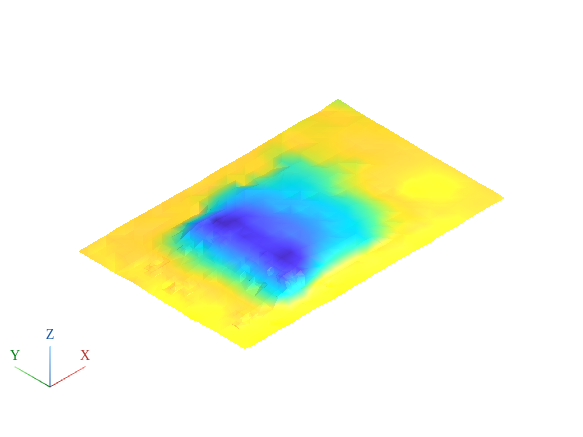
\includegraphics[width=\linewidth]{figs/A10.png}
  \caption{\textbf{Target A Reconstruction, 10 Frames}}
  \label{fig:A10Mesh}
\end{minipage}%
\begin{minipage}{.5\textwidth}
  \centering
  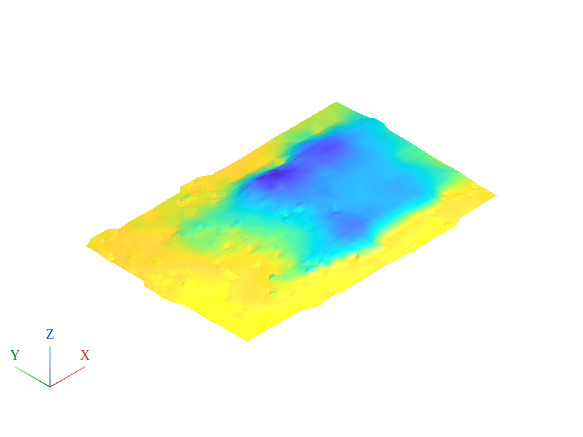
\includegraphics[width=\linewidth]{figs/B15.png}
  \caption{\textbf{Target B Reconstruction, 15 Frames}}
  \label{fig:B15Mesh}
\end{minipage}
\end{figure}
%----------------------------------------------------

%----------------------------------------------------
\begin{figure}[H]
\centering
\begin{minipage}{.5\textwidth}
  \centering
  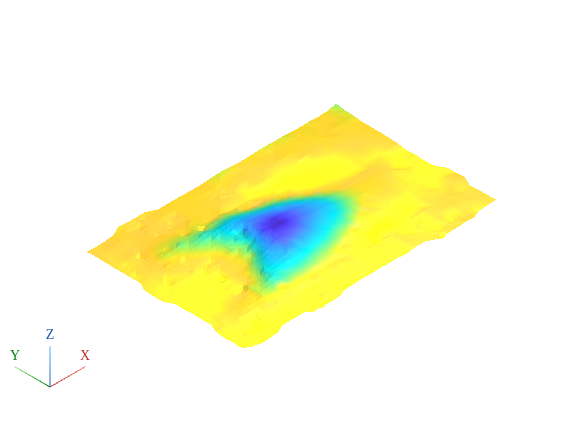
\includegraphics[width=\linewidth]{figs/C15.png}
  \caption{\textbf{Target C Reconstruction, 15 Frames}}
  \label{fig:C15Mesh}
\end{minipage}%
\begin{minipage}{.5\textwidth}
  \centering
  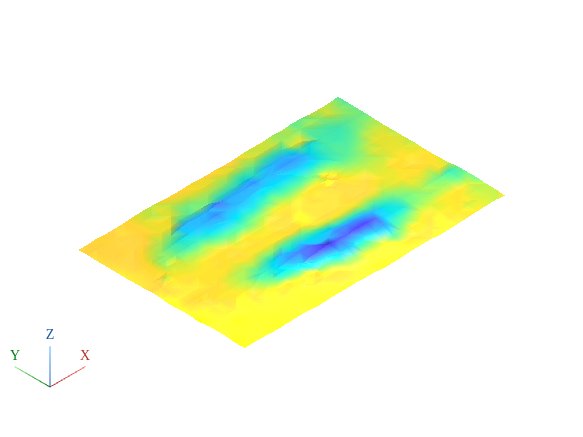
\includegraphics[width=\linewidth]{figs/D10.png}
  \caption{\textbf{Target D Reconstruction, 10 Frames}}
  \label{fig:D10Mesh}
\end{minipage}
\end{figure}
%----------------------------------------------------

%----------------------------------------------------
\subsection{Normals Estimation}
\label{subsec:ch7.section1.subsec2}

The normals estimation process made use of the reconstructed targets from the previous section with the highest point density available to allow for the most accurate normals estimation possible. For ease of visualisation, every fifth point's normal vector is displayed in the following figures.

The normals estimation process successfully calculated normal vectors for each point in the four reconstructed targets. The normal vectors generally point outwards from the surfaces of the targets, as expected. Besides a few inverted normals, their orientations were consistent with the overall reconstructions of the targets, as seen in the preceding section.

%----------------------------------------------------
\begin{figure}[H]
\centering
\begin{minipage}{.5\textwidth}
  \centering
  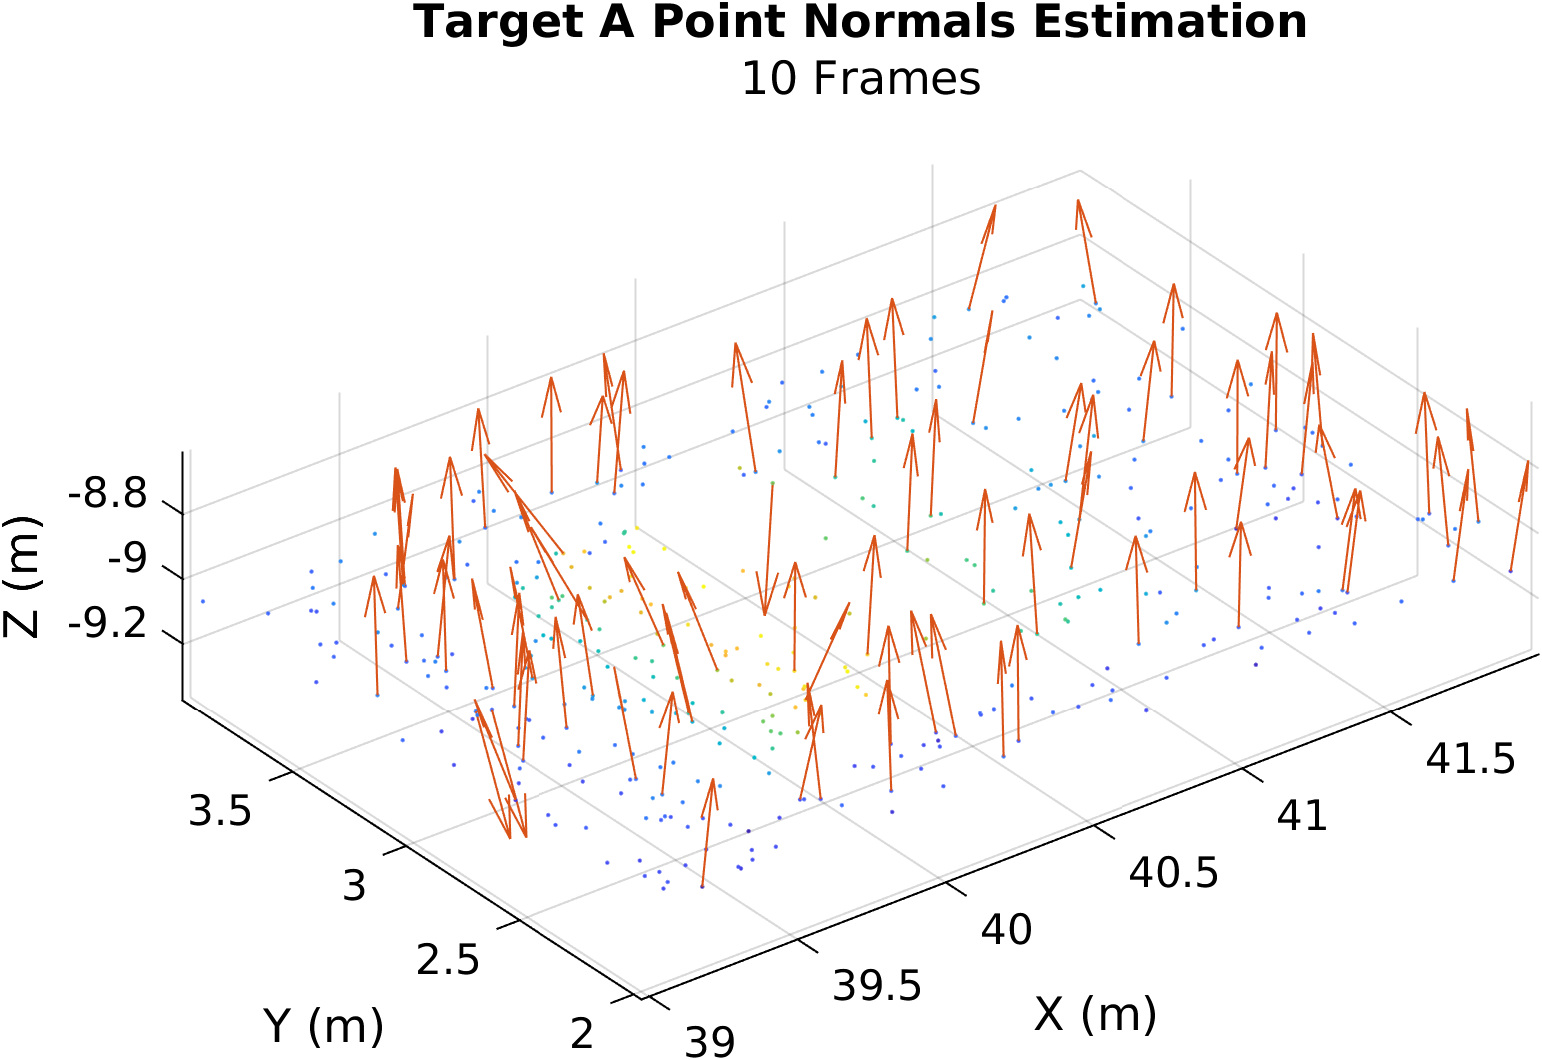
\includegraphics[width=0.95\linewidth]{figs/aNorm.png}
  \caption{\textbf{Target A}}
  \label{fig:A10Norm}
\end{minipage}%
\begin{minipage}{.5\textwidth}
  \centering
  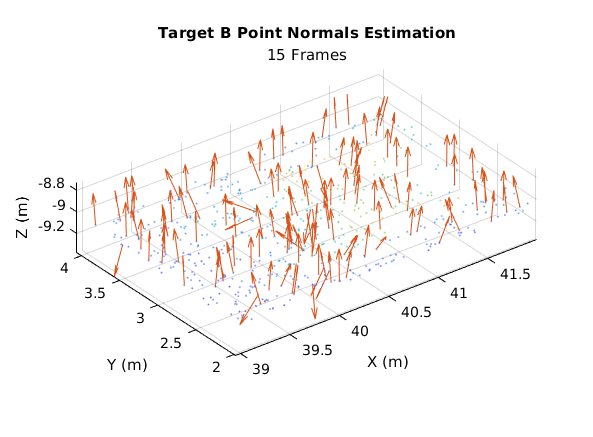
\includegraphics[width=0.95\linewidth]{figs/bNorm.png}
  \caption{\textbf{Target B}}
  \label{fig:B15Norm}
\end{minipage}
\end{figure}
%----------------------------------------------------

%----------------------------------------------------
\begin{figure}[H]
\centering
\begin{minipage}{.5\textwidth}
  \centering
  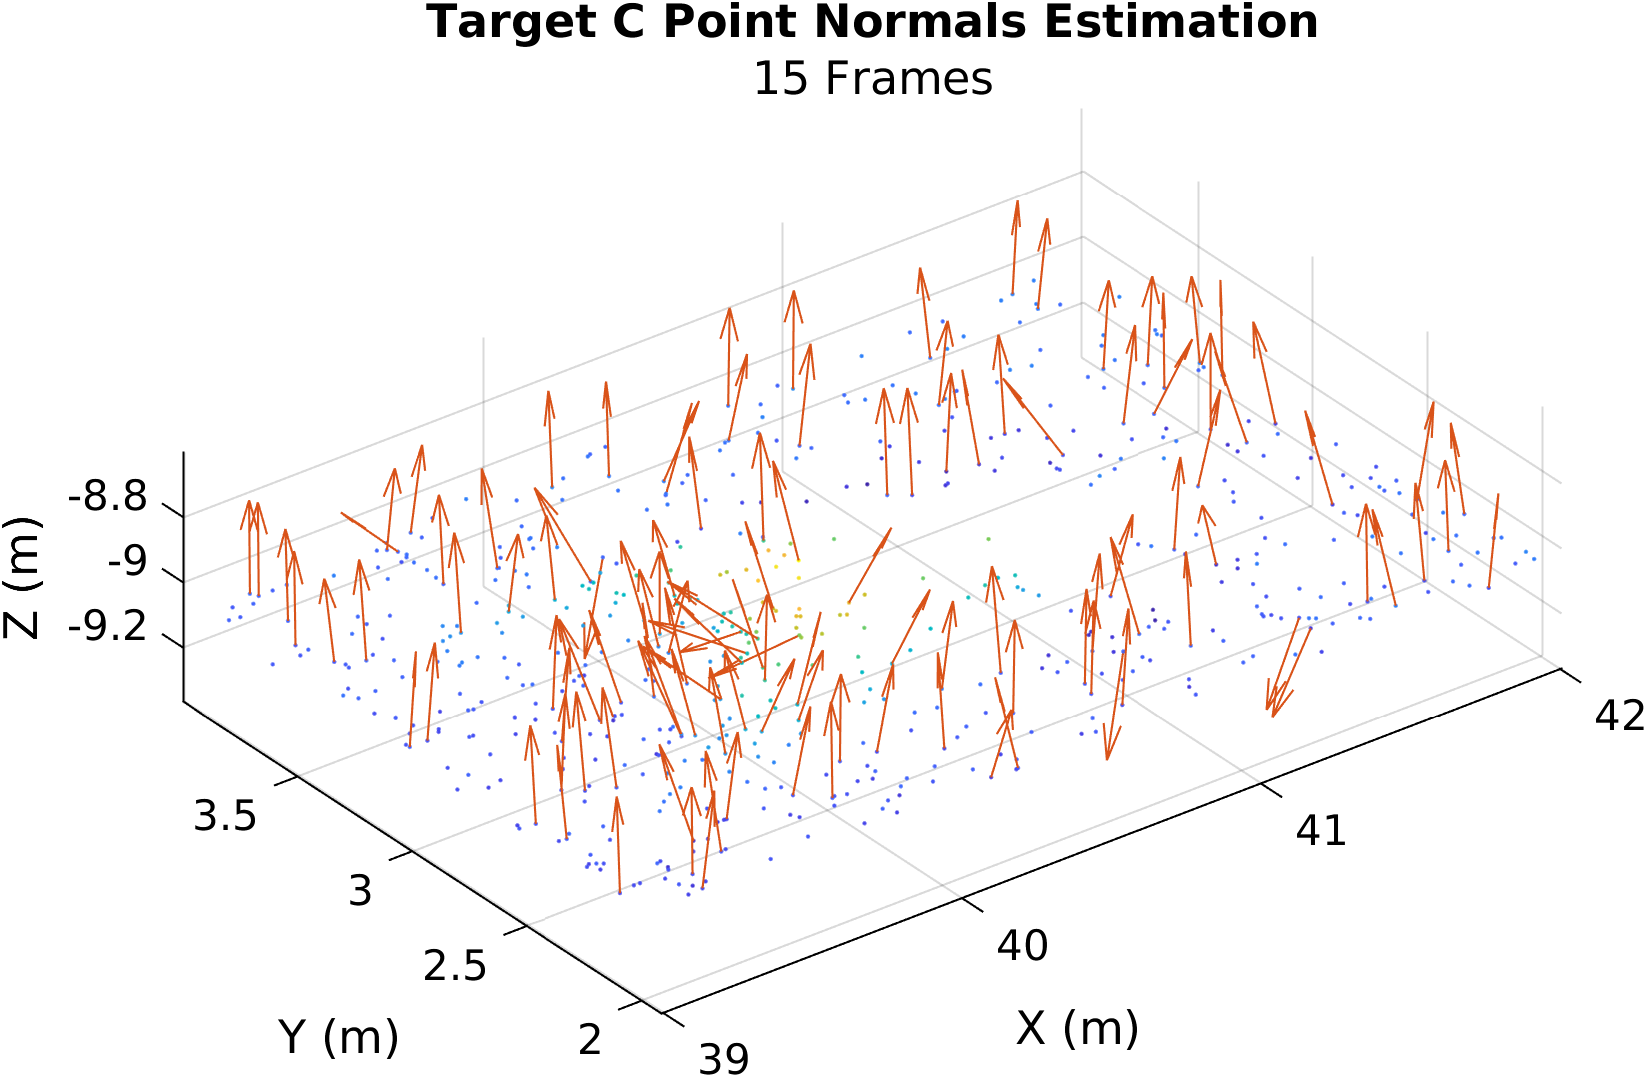
\includegraphics[width=0.95\linewidth]{figs/cNorm.png}
  \caption{\textbf{Target C}}
  \label{fig:C15Norm}
\end{minipage}%
\begin{minipage}{.5\textwidth}
  \centering
  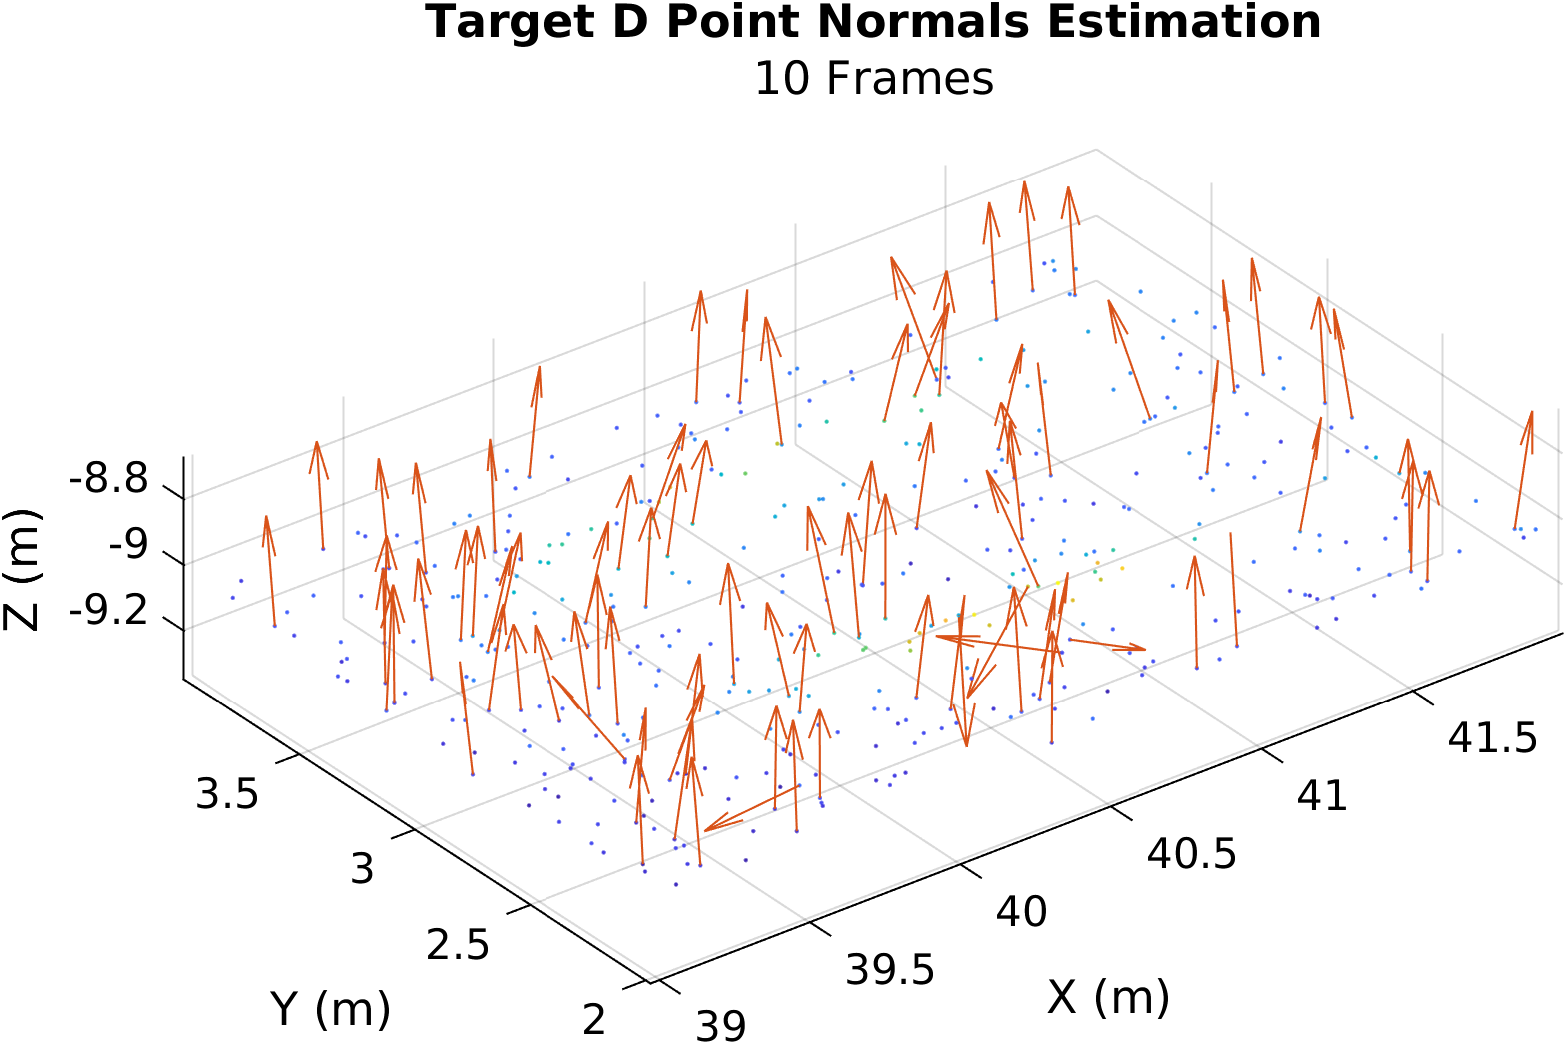
\includegraphics[width=0.95\linewidth]{figs/dNorm.png}
  \caption{\textbf{Target D}}
  \label{fig:D10Norm}
\end{minipage}
\end{figure}
%----------------------------------------------------

\newpage
%====================================================
\section{Motion Compensation and de-noising}
\label{sec:ch7.section2}
%----------------------------------------------------

%----------------------------------------------------
\subsection{Motion Compensation}
\label{subsec:ch7.section2.subsec1}

The motion capture system provided attitude data starting from initial angles of (0, 0, 0) for roll, pitch and yaw respectively, not taking into account the initial orientation of the Stewart platform and the Avia mounted to it. However, the Avia's \ac{IMU} provided data relative to its initial orientation at the start of data collection. This results in an offset between the two datasets, but does not impact the results and analysis of the experiment, as the relative motion is the focus of the experiment. To account for this offset, the initial roll and pitch angle offsets were removed from the angle estimations produced by both Kalman filters. For the first test (10° sweeps), the initial roll and pitch offsets were determined to be -1.6° and -2.075° respectively for both filters. For the second test (5° sweeps), the initial roll and pitch offsets were determined to be -1.625° and -1.95° for the Kalman filter and -1.585° and -2.175° for the \ac{ESKF}. 
\\*moved this paragraph from \ref{sec:ch5.section1}, still not 100\% sure*

The two implemented Kalman filters, both produced reasonable roll and pitch angle estimates for motion compensation of the \ac{LiDAR} point cloud data. The \ac{ESKF} and \ac{KF}  produced angle estimates very similar to each other, see Figures \ref{fig:vs_roll_10}, \ref{fig:vs_pitch_10}, \ref{fig:vs_roll_5} and \ref{fig:vs_pitch_5}. The \ac{KF} tended to overestimate the angles slightly more than the \ac{ESKF}, particularly in the 10° sweep test, see Figures \ref{fig:resid_10} and \ref{fig:resid_5}. For both the 10° and 5° sweep tests, the \ac{ESKF} had slightly more variability in its angle estimates compared to the \ac{KF}, which produced smoother angle estimates. For both sweep tests, particularly the 5° sweep test the pitch angle estimates from both filters appeared to track the true pitch motion more closely than the roll estimates, which exhibited larger deviations from the true roll motion.

When the angle estimates from both filters were used to motion compensate the \ac{LiDAR} point cloud data, both filters produced similar results in terms of reducing motion-induced distortions. Visual inspection of the compensated point clouds indicated that both filters were effective at reducing distortions, with no significant differences in the overall quality of the compensated point clouds. Artefacts and distortions induced by yaw motion, translation and high-frequency vibrations were not addressed by either filter, as expected.

%----------------------------------------------------
\subsubsection{10° Sweep Test}
\label{subsec:ch7.section2.subsec1.subsubsec1}

%----------------------------------------------------
\begin{figure}[H]
    \centering
    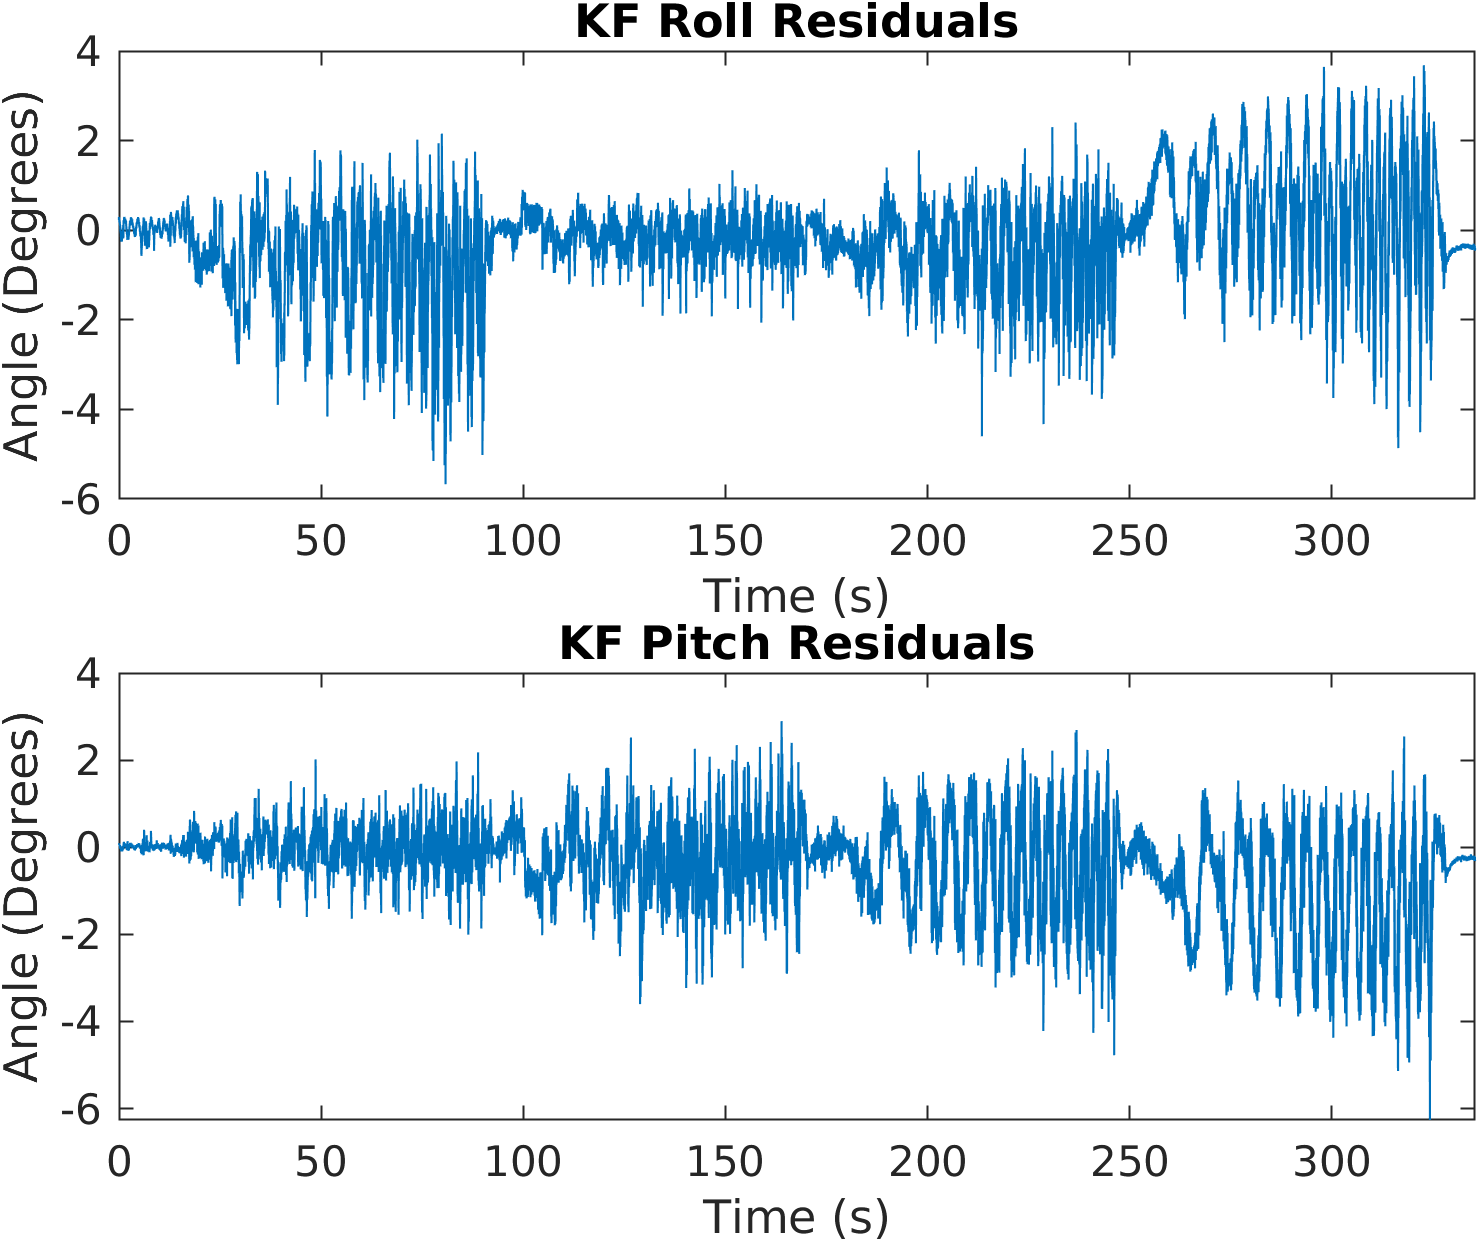
\includegraphics[width=0.85\textwidth]{figs/kf_resid_10.png}
    \caption{\textbf{KF residuals}}
    \label{fig:kf_resid_10}
\end{figure}
%----------------------------------------------------

%----------------------------------------------------
\begin{figure}[H]
    \centering
    
\includegraphics[width=0.85\textwidth]{figs/eskf_resid_10.png}
    \caption{\textbf{ESKF residuals}}
    \label{fig:eskf_resid_10}
\end{figure}
%----------------------------------------------------

%----------------------------------------------------
\begin{figure}[H]
    \centering
    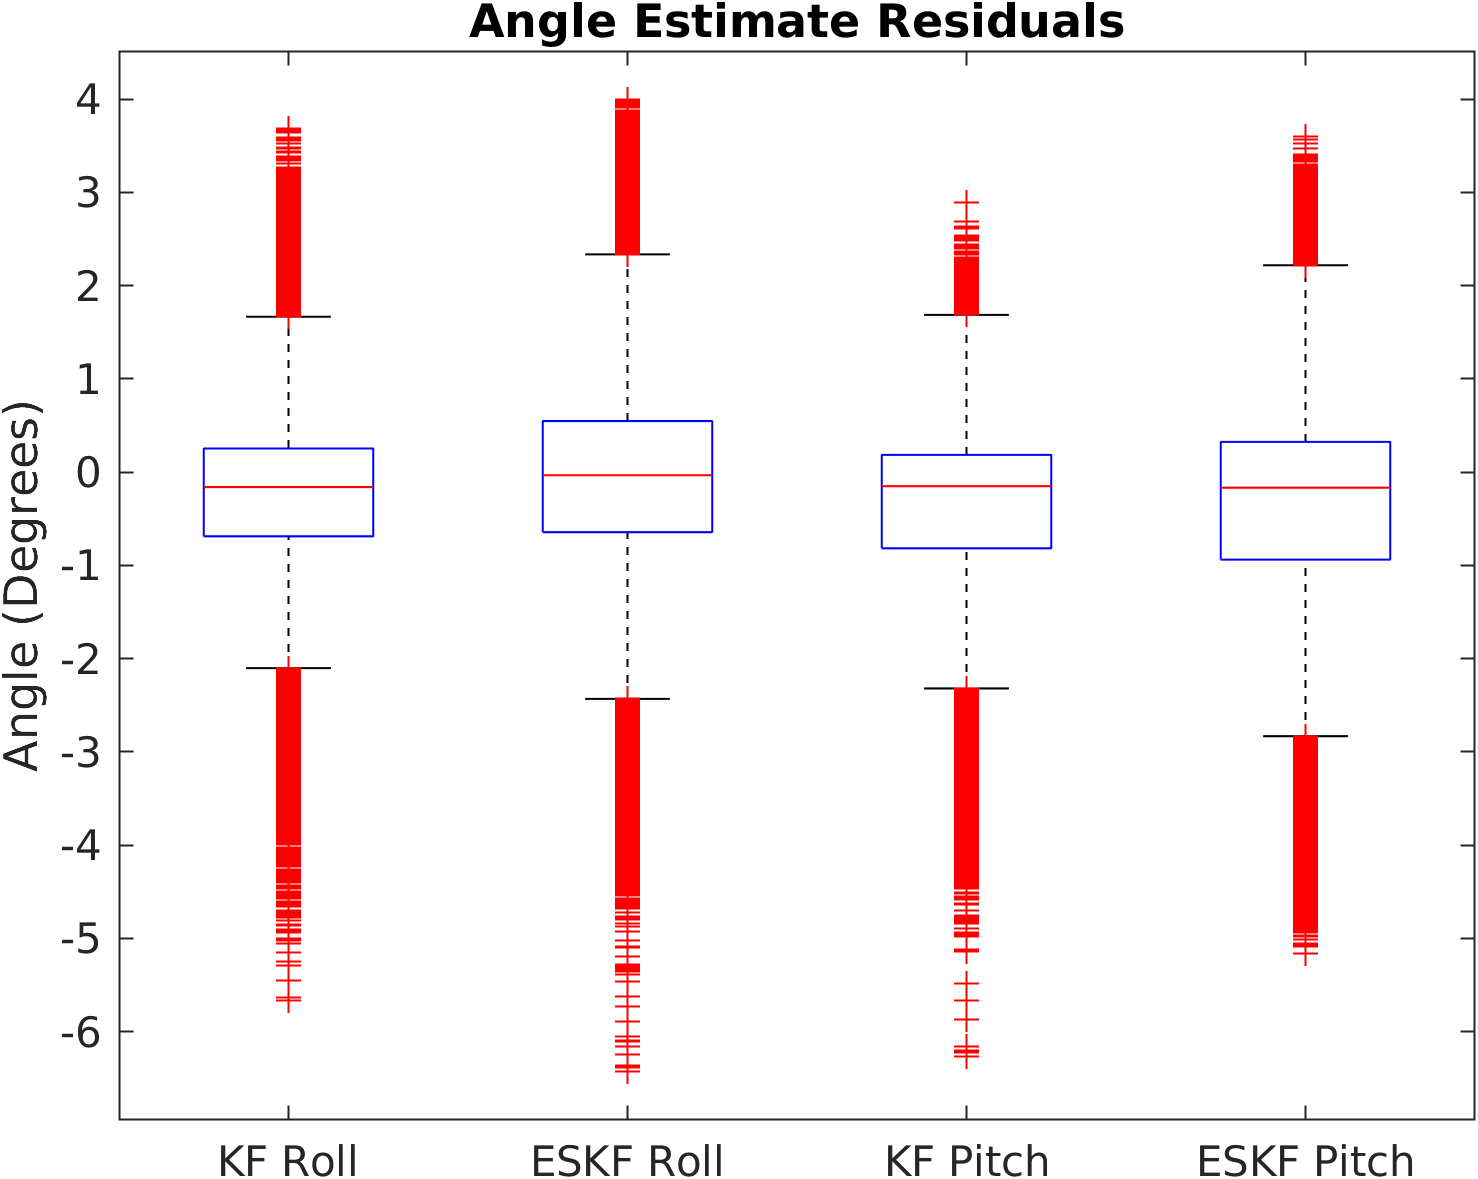
\includegraphics[width=0.85\textwidth]{figs/vs_resids_10.png}
    \caption{\textbf{residuals}}
    \label{fig:resid_10}
\end{figure}
%----------------------------------------------------

\newpage

%----------------------------------------------------
\subsubsection{5° Sweep Test}
\label{subsec:ch7.section2.subsec1.subsubsec2}

%----------------------------------------------------
\begin{figure}[H]
    \centering
    
\includegraphics[width=0.85\textwidth]{figs/kf_resid_5.png}
    \caption{\textbf{KF residuals}}
    \label{fig:kf_resid_5}
\end{figure}
%----------------------------------------------------

%----------------------------------------------------
\begin{figure}[H]
    \centering
    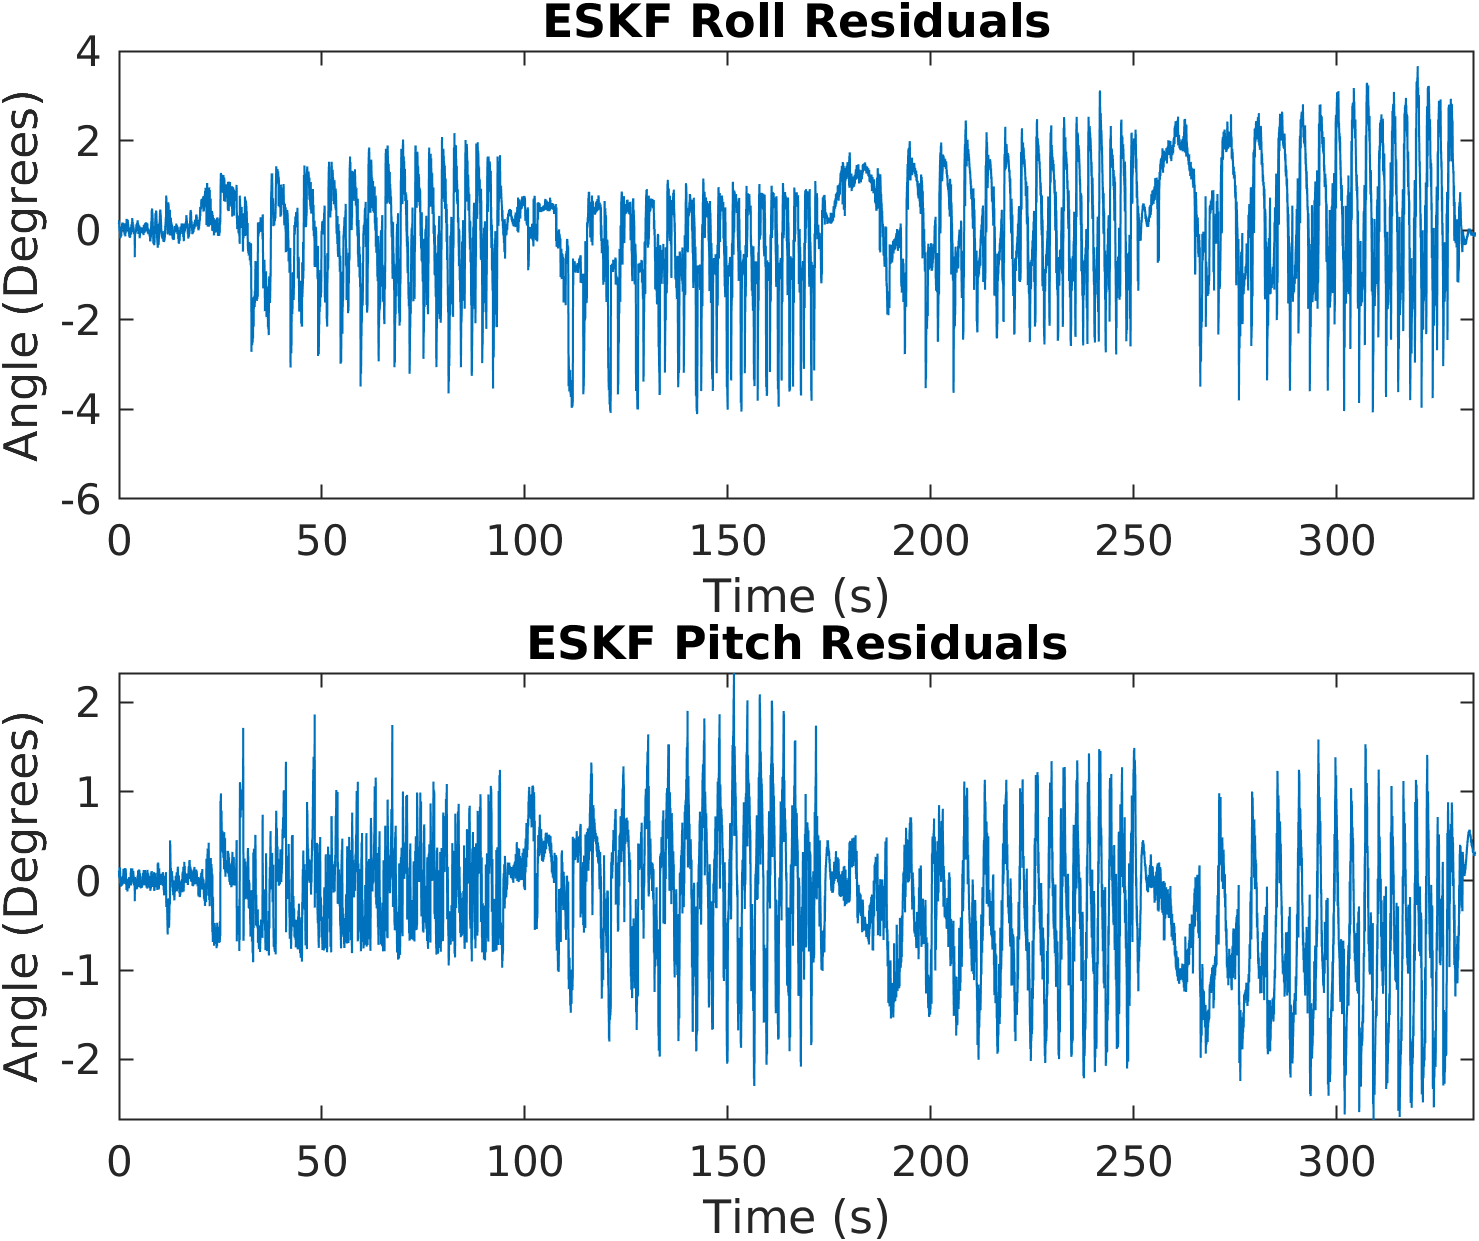
\includegraphics[width=0.85\textwidth]{figs/eskf_resid_5.png}
    \caption{\textbf{ESKF residuals}}
    \label{fig:eskf_resid_5}
\end{figure}
%----------------------------------------------------

%----------------------------------------------------
\begin{figure}[H]
    \centering
    
\includegraphics[width=0.85\textwidth]{figs/vs_resids_5.png}
    \caption{\textbf{residuals}}
    \label{fig:resid_5}
\end{figure}
%----------------------------------------------------

%----------------------------------------------------
\begin{figure}[H]
    \centering
    
\includegraphics[width=\textwidth]{figs/scale_attitude.png}
    \caption{\textbf{Attitude Estimation.} Avia attitude estimation made by ESKF during SCALE cruise, 24 July 2022.}
    \label{fig:scale_attitude}
\end{figure}
%----------------------------------------------------

\newpage

%----------------------------------------------------
\subsection{De-noising}
\label{subsec:ch7.section2.subsec2}

The de-noising function performed as expected. It removes unwanted returns produced by adverse environmental conditions without removing many valid points from the target scene.

%----------------------------------------------------
\begin{figure}[H]
    \centering
    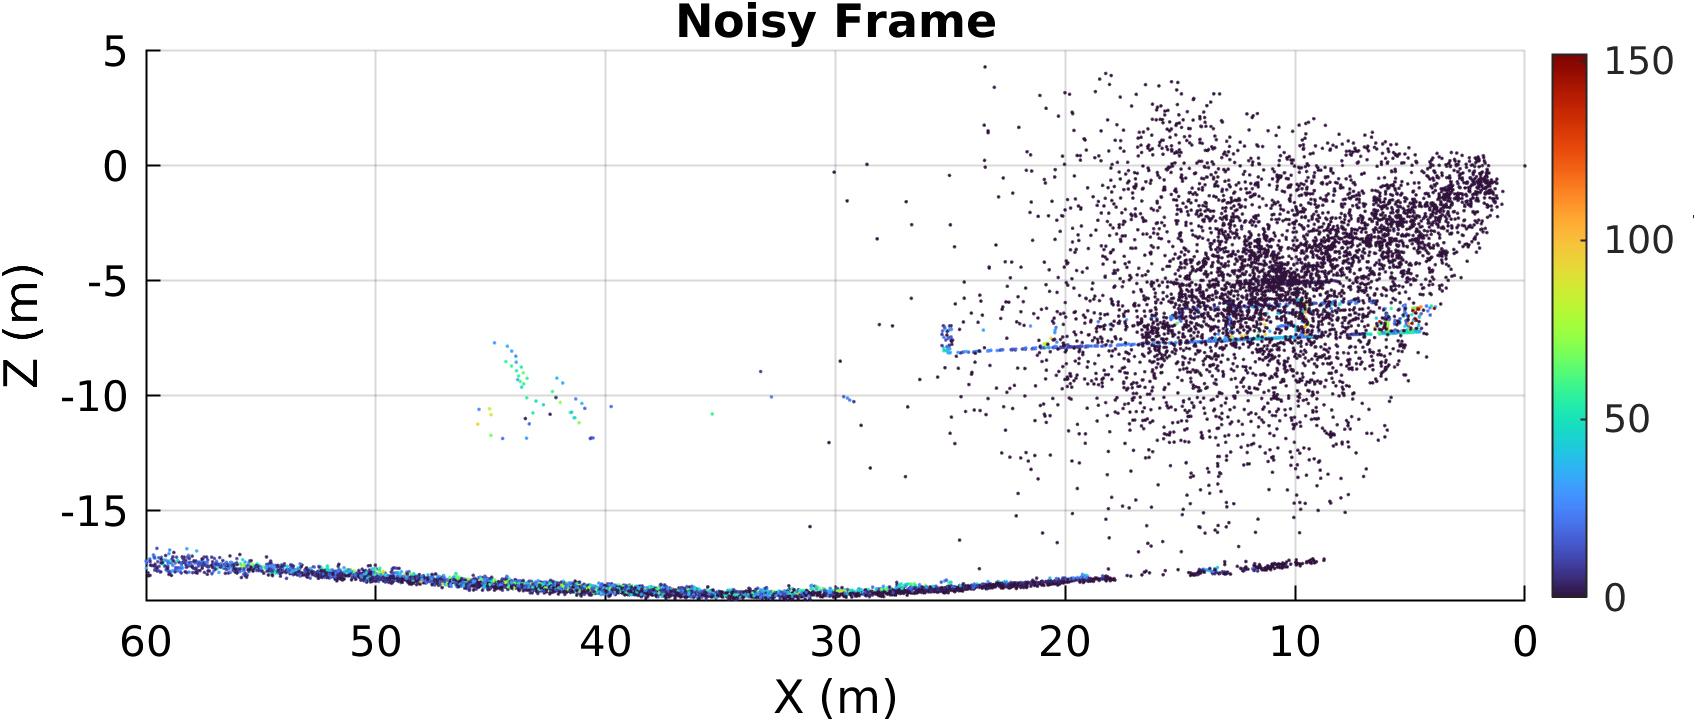
\includegraphics[width=0.9\textwidth]{figs/no_threshold.png}
    \caption{\textbf{Noisy Frame}}
    \label{fig:no_thresh}
\end{figure}
%----------------------------------------------------

%----------------------------------------------------
\begin{figure}[H]
    \centering
    
\includegraphics[width=0.9\textwidth]{figs/threshold.png}
    \caption{\textbf{De-noised Frame}}
    \label{fig:thresh}
\end{figure}
%----------------------------------------------------

As seen in Figures \ref{fig:no_thresh} and \ref{fig:thresh} above, the cone of noisy data in front of the sensor's aperture has been removed, with minimal invalid points remaining in the region. The horizontal feature that remains is a part of the ship's deck from where the data was collected. A few points from the ice field have been removed by the process, as seen around Z = -20 m, X = 10 m in Figure \ref{fig:thresh}, but the vast majority of the ice field points have been preserved.

\newpage
%====================================================
\section{Wave Parameter Estimation}
\label{sec:ch7.section3}
%----------------------------------------------------

The mean wave magnitude and period were able to be determined with a high degree of confidence from the wave probe data using the MATLAB \emph{curveFitter} tool. All tests produced R-square scores above 0.93, indicating a strong correlation between the fitted model and the raw probe data, as seen in Table \ref{tab:curveFitter}. The wave periods all closely matched the parameters set to the wave makers (1.6 s and 2 s). *this needs to be corrected* However, the amplitudes did not match the set values as closely, the first, second and fifth tests tracked the set values fairly well, while the third, fourth and sixth tests did not. The third and fourth tests fitted amplitudes were significantly lower than the set value of 50 mm, while the sixth test fitted amplitude was marginally higher than the set value of 27.5 mm.

%----------------------------------------------------
\begin{figure}[H]
    \centering
    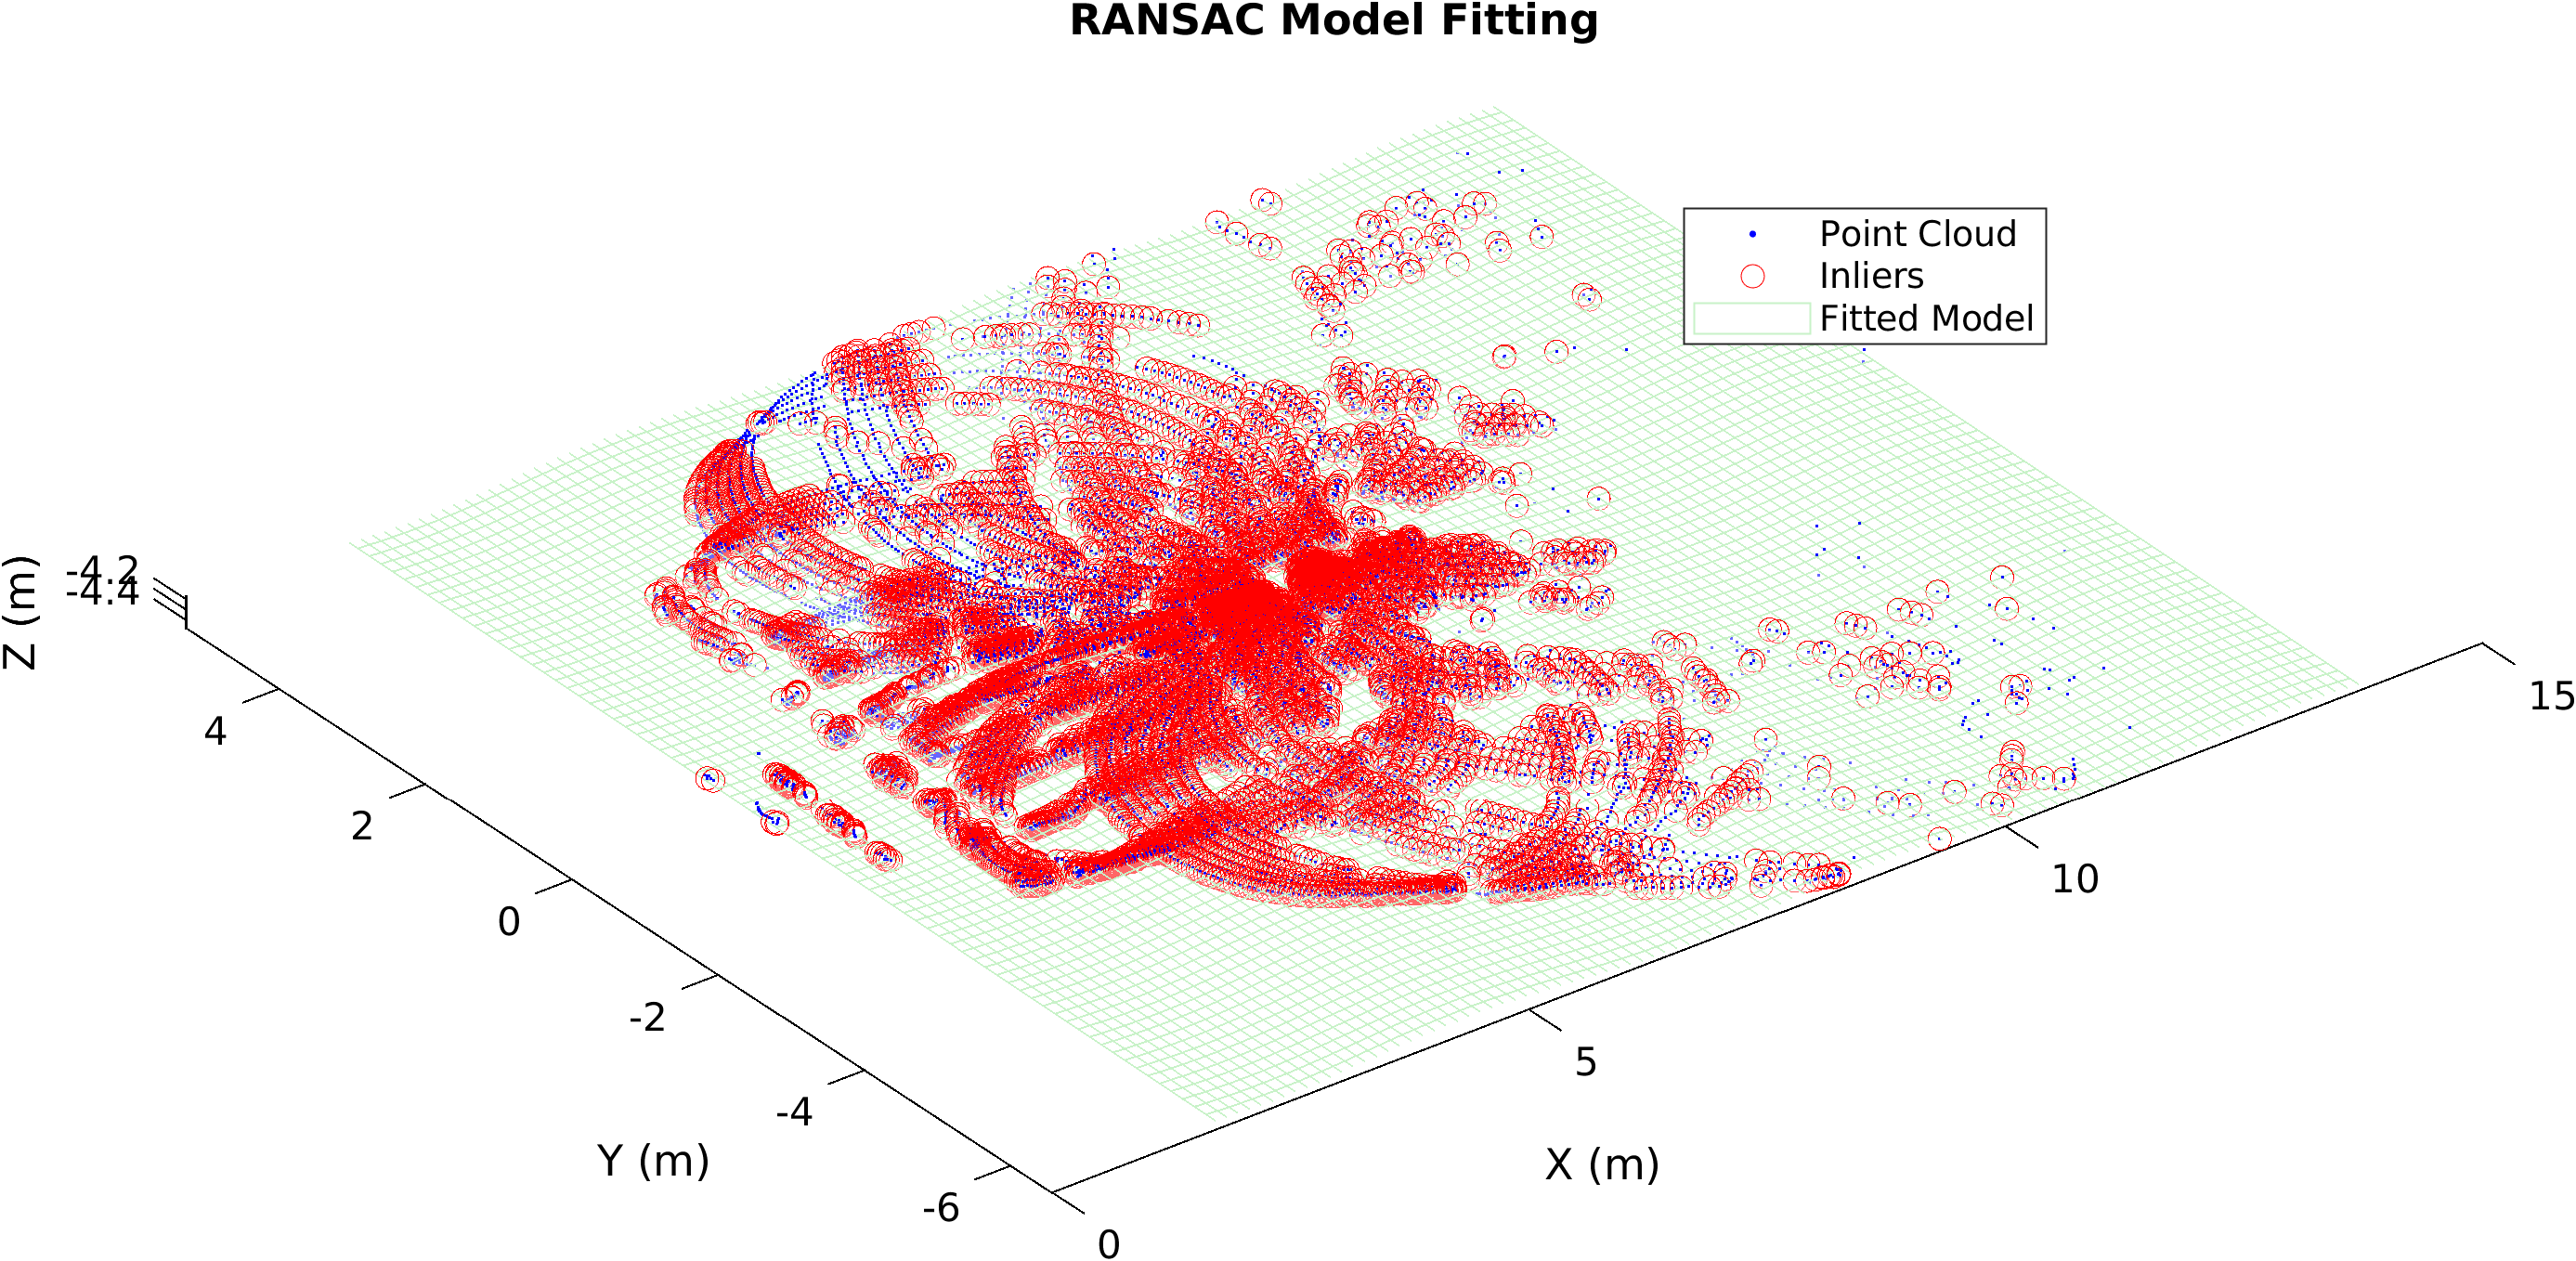
\includegraphics[width=0.6\textwidth]{figs/fit_view.png}
    \caption{\textbf{Fitted Wave Model}}
    \label{fig:fit_view}
\end{figure}
%----------------------------------------------------

%----------------------------------------------------
\begin{figure}[H]
    \centering
    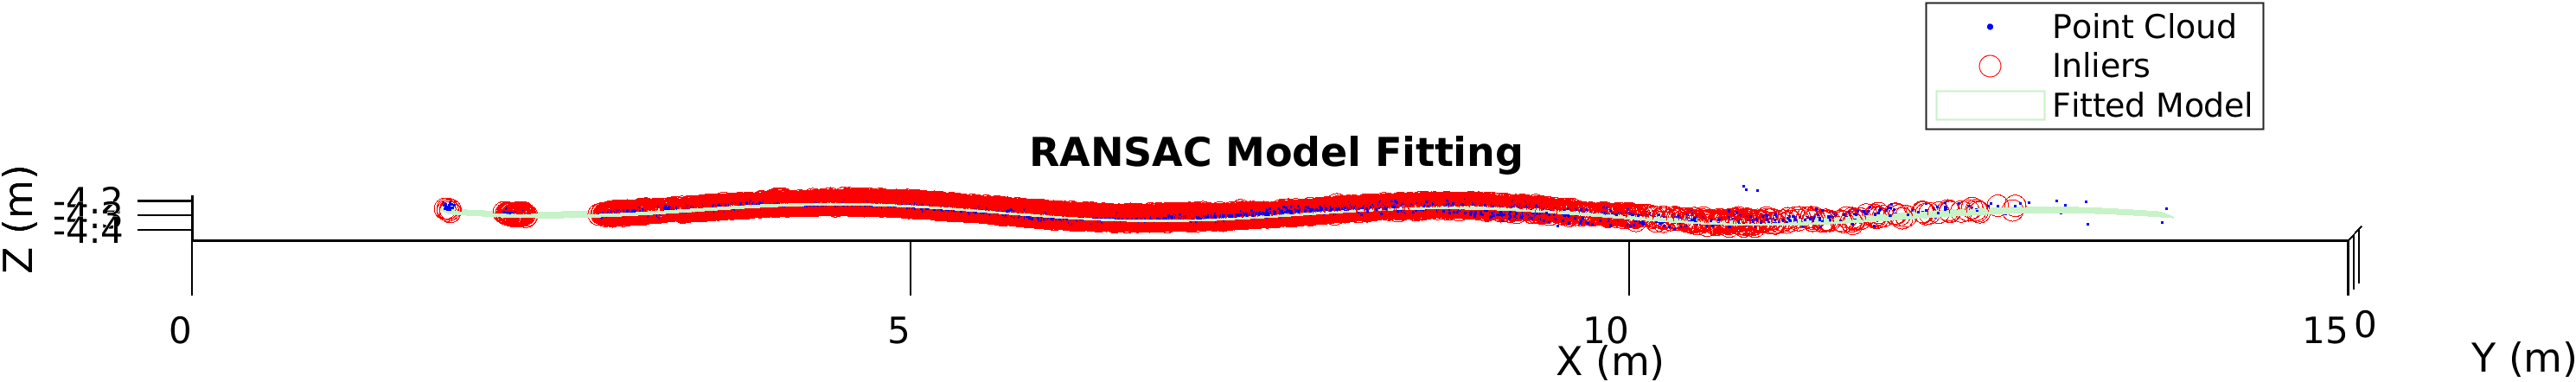
\includegraphics[width=\textwidth]{figs/fit_profile.png}
    \caption{\textbf{Fitted Wave Model}}
    \label{fig:fit_profile}
\end{figure}
%----------------------------------------------------

%----------------------------------------------------
\begin{table}[H]
\centering
\resizebox{\textwidth}{!}{%
\begin{tabular}{|l|c|c|c|c|}
\hline
\textbf{Test} &
  \multicolumn{1}{l|}{\textbf{Amplitude (mm)}} &
  \multicolumn{1}{l|}{\textbf{Angular Frequency (rad/s)}} &
  \multicolumn{1}{l|}{\textbf{Calculated Period (s)}} &
  \multicolumn{1}{l|}{\textbf{R-square Score}} \\ \hline
1 & 24.9046 & 3.9259 & 1.6004 & 0.98606 \\ \hline
2 & 35.1361 & 3.9259 & 1.6004 & 0.97659 \\ \hline
3 & 45.7627 & 3.9257 & 1.6005 & 0.96552 \\ \hline
4 & 40.9202 & 3.142  & 1.9997 & 0.96427 \\ \hline
5 & 34.1690 & 3.1443 & 1.9983 & 0.97534 \\ \hline
6 & 27.8620 & 3.1438 & 1.9986 & 0.93052 \\ \hline
\end{tabular}%
}
\caption{curveFitter Parameter Estimations}
\label{tab:curveFitter}
\end{table}
%----------------------------------------------------

%----------------------------------------------------
\begin{table}[H]
\centering
\resizebox{\textwidth}{!}{%
\begin{tabular}{|l|c|c|c|c|}
\hline
\textbf{Test} &
  \multicolumn{1}{l|}{\textbf{Mean Amplitude (mm)}} &
  \multicolumn{1}{l|}{\textbf{Mean Wave Number (rad/m)}} &
  \multicolumn{1}{l|}{\textbf{Calculated Mean Period (s)}} &
  \multicolumn{1}{l|}{\textbf{Mean Inliers}} \\ \hline
1 & 26.0053 & 1.5404 & 1.6185 & 80.79 \%  \\ \hline
2 & 37.3767 & 1.5566 & 1.6093 & 75.81 \%  \\ \hline
3 & 47.8268 & 1.5518 & 1.6119 & 72.28 \%  \\ \hline
4 & 55.3504 & 1.0039 & 2.0037 & 67.33 \%  \\ \hline
5 & 43.2641 & 1.0079 & 2.0001 & 69.15 \%  \\ \hline
6 & 29.3343 & 1.0137 & 1.9944 & 72.06 \% \\ \hline
\end{tabular}%
}
\caption{\ac{RANSAC} Parameter Estimations}
\label{tab:RANSAC}
\end{table}
%----------------------------------------------------

%----------------------------------------------------
\begin{figure}[H]
\centering
\begin{minipage}{.5\textwidth}
  \centering
  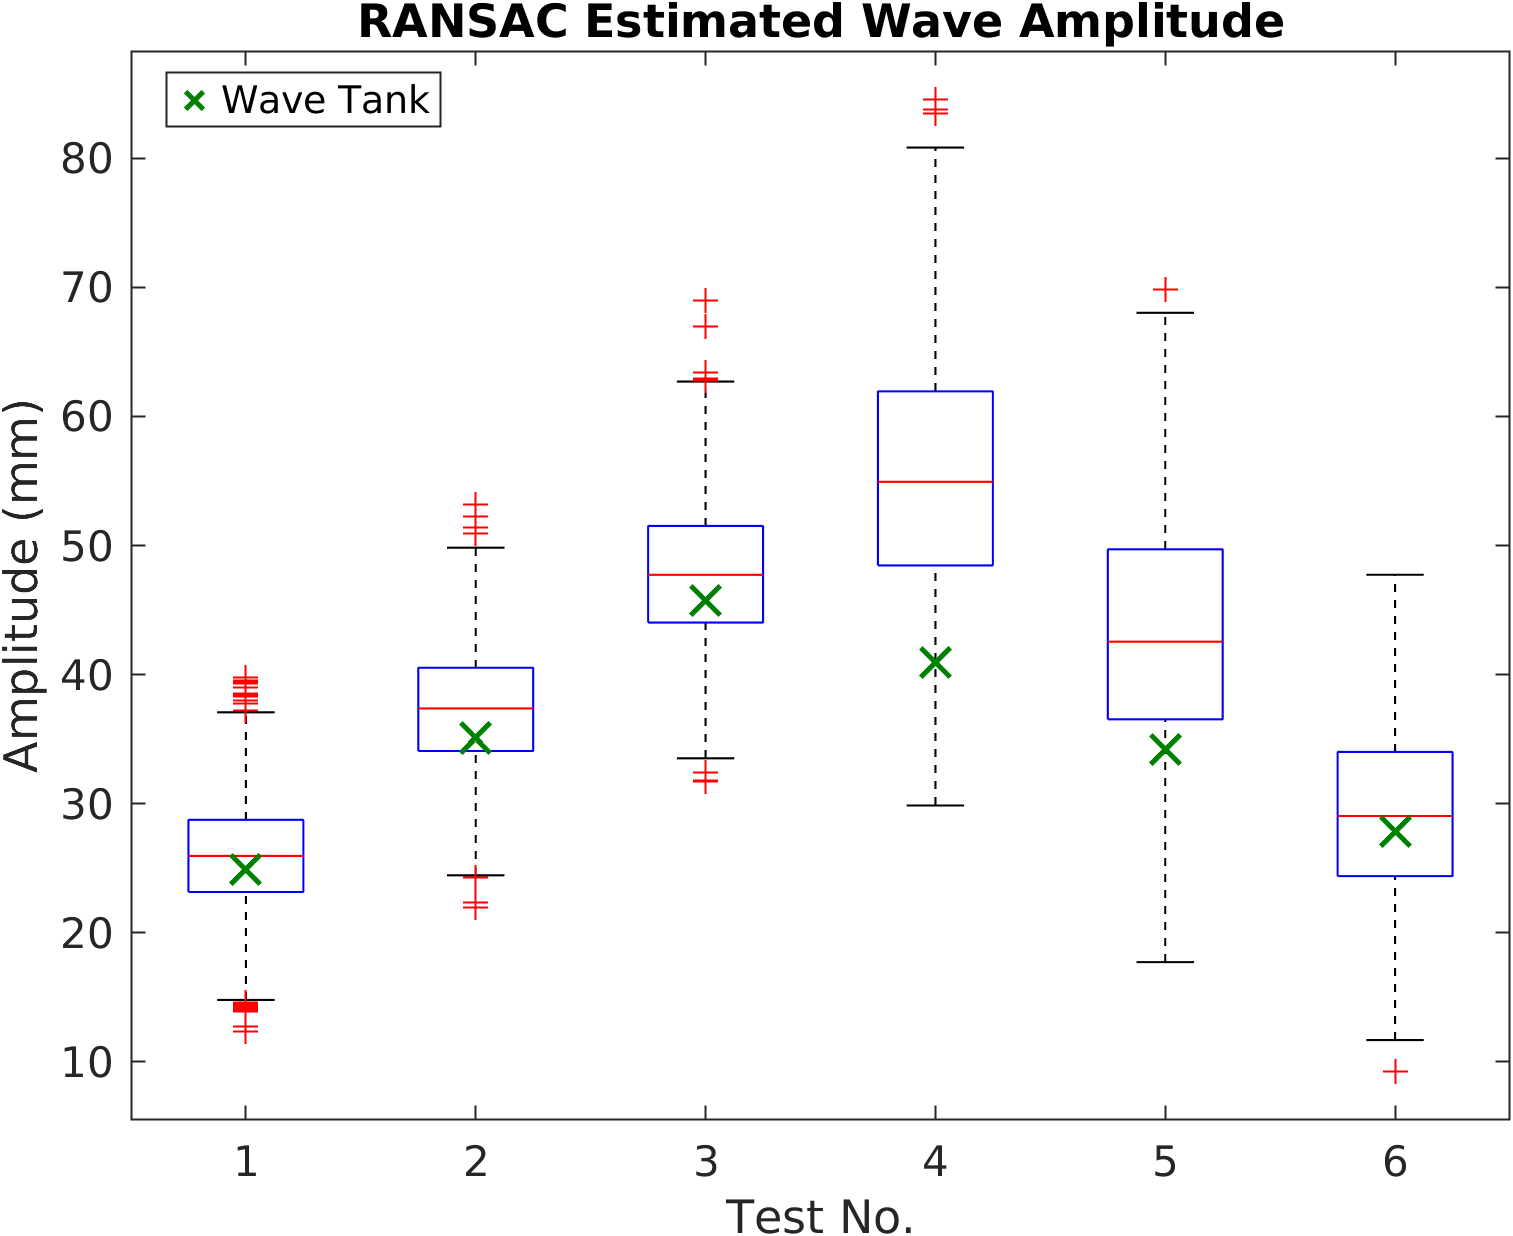
\includegraphics[width=\linewidth]{figs/ransac_amp_truth.png}
  \caption{\textbf{Estimated Amplitude}}
  \label{fig:amp}
\end{minipage}%
\begin{minipage}{.5\textwidth}
  \centering
  
\includegraphics[width=\linewidth]{figs/ransac_period_truth.png}
  \caption{\textbf{Estimated Period}}
  \label{fig:period}
\end{minipage}
\end{figure}
%----------------------------------------------------

The wave parameters estimated from the \ac{LiDAR} point cloud data using the \ac{RANSAC} method, seen in Table \ref{tab:RANSAC}, provided mixed, but mostly positive results. All fitted \ac{RANSAC} models had over 65\% mean inliers and only two tests (four and five) has less than 72\% mean inliers. The calculated mean periods very closely matched the wave probe data (see Figure \ref{fig:period}), with the greatest difference being 0.0181 s in the first test. In all cases the estimated mean periods were greater than the probe data values.
The estimated mean amplitudes matched the probe data results fairly well in the first three and last tests, with the greatest difference being 2.2406 mm in the second test. However, for the last fourth and fifth tests, the estimated mean amplitudes were significantly higher than the probe data values, with the fourth test value 14.4302 mm and fifth test value 9.0951 mm greater than their respective probe data values (see Figure \ref{fig:amp}).

In every test, the higher the percentage of mean inliers in the model estimation, the closer the match between the estimated \ac{RANSAC} wave parameters and the probe data wave parameters.

%----------------------------------------------------
\begin{figure}[H]
\centering
\begin{minipage}{.5\textwidth}
  \centering
  
\includegraphics[width=\linewidth]{figs/rand_amp.png}
  \caption{\textbf{Estimated Amplitude, 5 Samples}}
  \label{fig:rand_amp}
\end{minipage}%
\begin{minipage}{.5\textwidth}
  \centering
  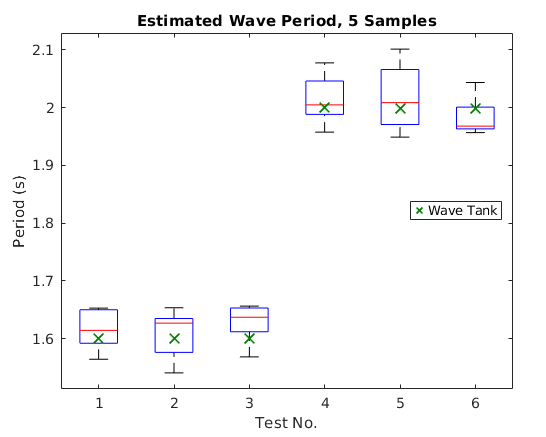
\includegraphics[width=\linewidth]{figs/rand_per.png}
  \caption{\textbf{Estimated Period, 5 Samples}}
  \label{fig:rand_period}
\end{minipage}
\end{figure}
%----------------------------------------------------

To investigate the accuracy of the \ac{RANSAC} wave parameter estimations from limited data samples, five random samples of the estimated amplitude and period from each test were taken, as seen in Figures \ref{fig:rand_amp} and \ref{fig:rand_period}. The results show that even with a limited number of samples, the estimated wave parameters closely match the overall estimated values from Table \ref{tab:RANSAC}.

\newpage
%====================================================
\section{Pancake Identification \& Clustering}
\label{sec:ch7.section4}
%----------------------------------------------------

In each scene, the three clustering algorithms were applied to both the single frame and two frames concatenated point cloud targets. The results were then visually inspected to determine if any distinct pancake clusters were identified by each algorithm. The number of points in the two largest or most distinct clusters identified by each algorithm in each scene were recorded for comparison. Any major differences in cluster shapes or distributions were also noted.

%----------------------------------------------------
\subsection{Scene 1 - 19 July 2022}
\label{subsec:ch7.section4.subsec1}

When visually inspecting the point cloud data and video data from this scene, it was hypothesised that it would be an ideal candidate for clustering due to the visible pancake floes in the video footage and relatively consistent point density in the point cloud data. However, all three algorithms failed to identify distinct pancake clusters in either the single frame or two frame concatenated targets.

%----------------------------------------------------
\begin{figure}[H]
\centering
\begin{minipage}{.5\textwidth}
  \centering
  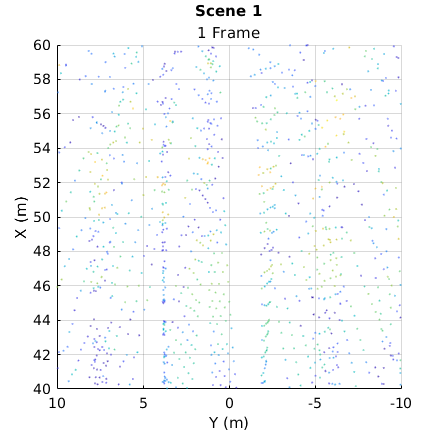
\includegraphics[width=0.95\linewidth]{figs/2290frame.png}
  \caption{\textbf{Scene 1, 1 Frame}}
  \label{fig:2290Frame}
\end{minipage}%
\begin{minipage}{.5\textwidth}
  \centering
  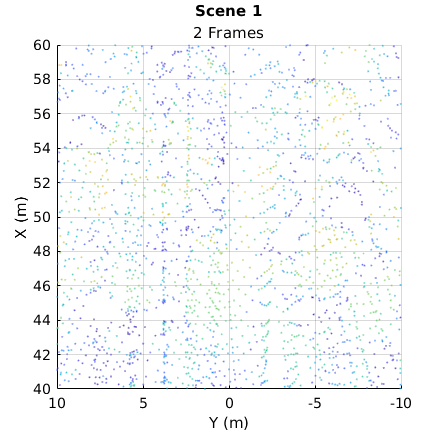
\includegraphics[width=0.95\linewidth]{figs/2291frame.png}
  \caption{\textbf{Scene 1, 2 Frames}}
  \label{fig:2291Frame}
\end{minipage}
\end{figure}
%----------------------------------------------------

%----------------------------------------------------
\begin{figure}[H]
    \centering
    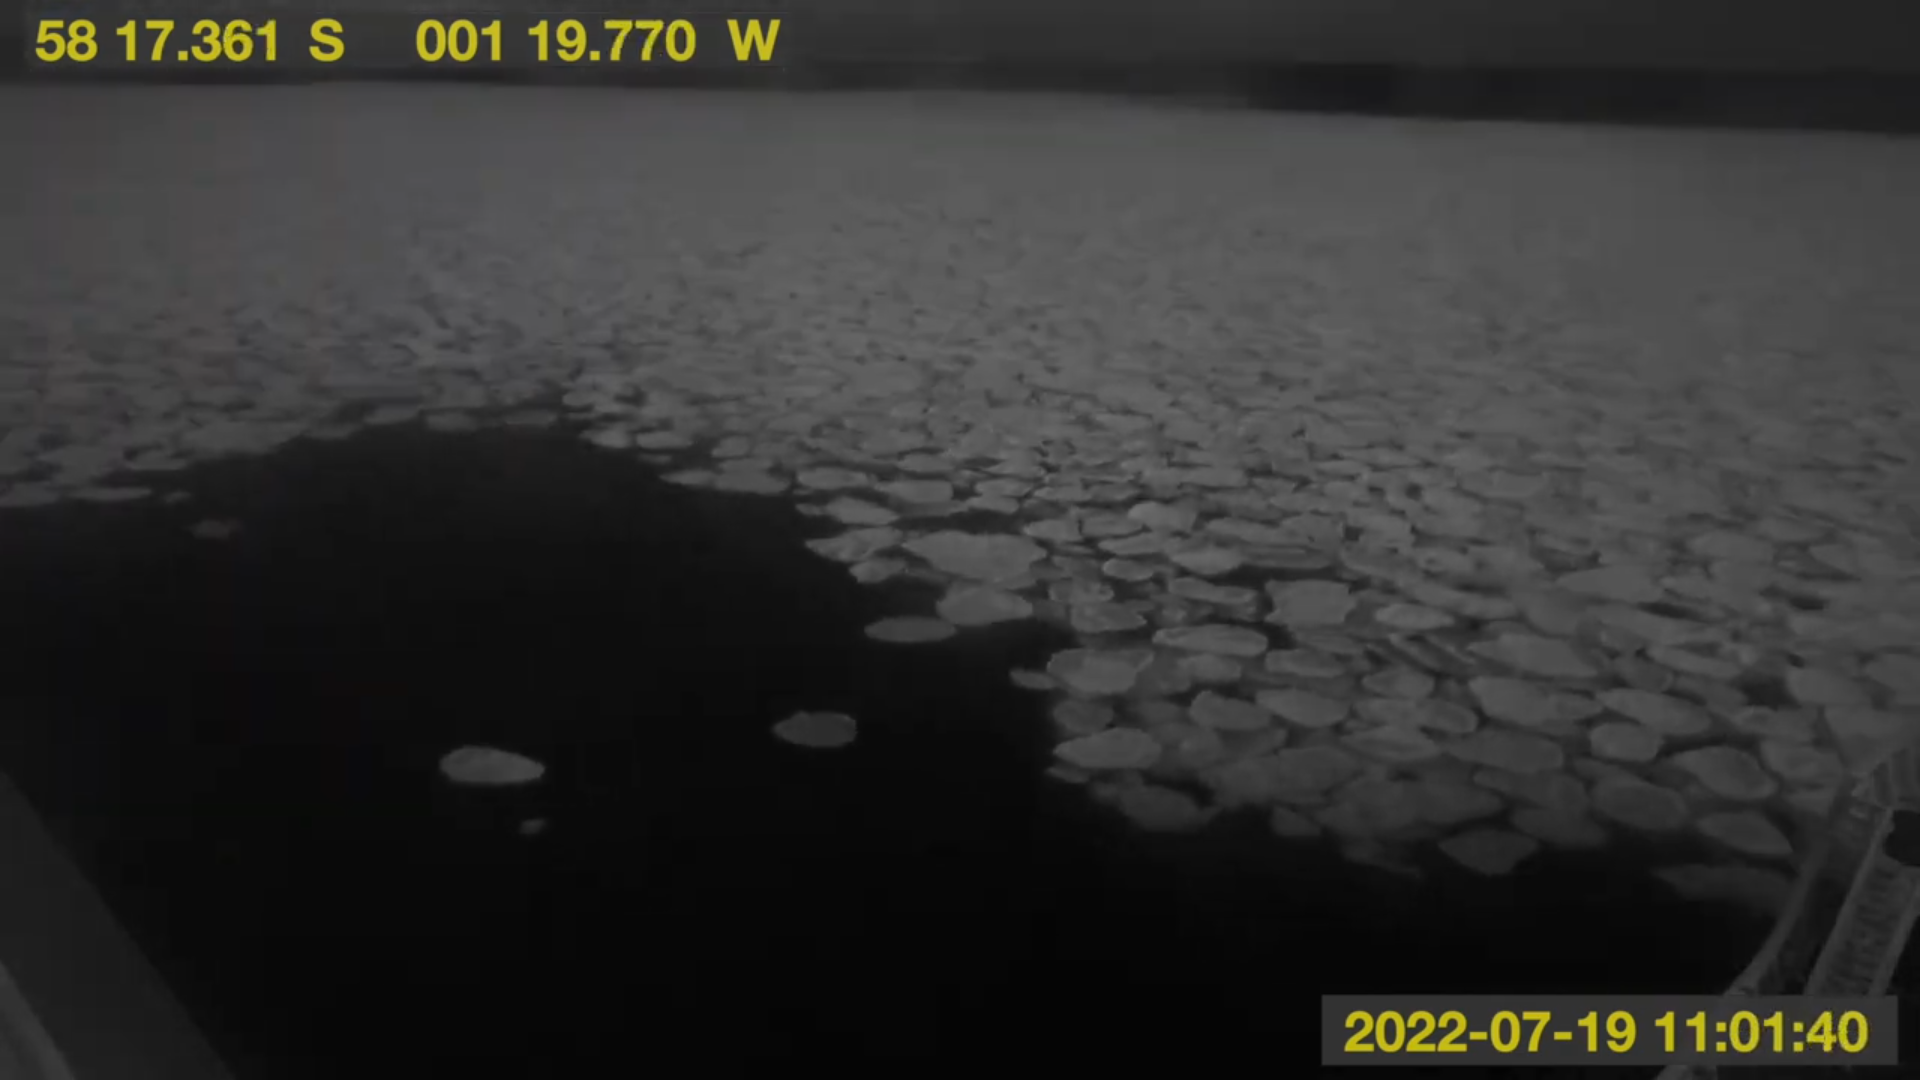
\includegraphics[width=0.8\textwidth]{figs/2290cam.PNG}
    \caption{\textbf{Scene 1 Video Still}}
    \label{fig:2290}
\end{figure}
%----------------------------------------------------

%----------------------------------------------------
\subsection{Scene 2 - 23 July 2022}
\label{subsec:ch7.section4.subsec2}

Cluster A is the teal group above the centre and cluster B is the orange group below group A in Figure \ref{fig:clust660DB}. These two clusters were identified by \ac{DBScan} and \ac{OPTICS} in both single frame and two frame concatenated targets. \ac{VDBScan} failed to identify any clusters in either target.

%----------------------------------------------------
\begin{table}[H]
\centering
\begin{tabular}{|l|l|r|c|r|}
\hline
\textbf{No Frames} & \textbf{Cluster} & \multicolumn{1}{l|}{\textbf{DBScan}} & \multicolumn{1}{l|}{\textbf{VDBScan}} & \multicolumn{1}{l|}{\textbf{OPTICS}} \\ \hline
\multirow{2}{*}{1} & A                & 188                                  & NaN                                   & 181                                  \\ \cline{2-5} 
                   & B                & 194                                  & NaN                                   & 178                                  \\ \hline
\multirow{2}{*}{2} & A                & 351                                  & NaN                                   & 347                                  \\ \cline{2-5} 
                   & B                & 363                                  & NaN                                   & 385                                  \\ \hline
\end{tabular}
\caption{Scene 1 Points per Cluster}
\label{tab:660Clust}
\end{table}
%----------------------------------------------------

%----------------------------------------------------
\begin{figure}[H]
\centering
\begin{minipage}{.5\textwidth}
  \centering
  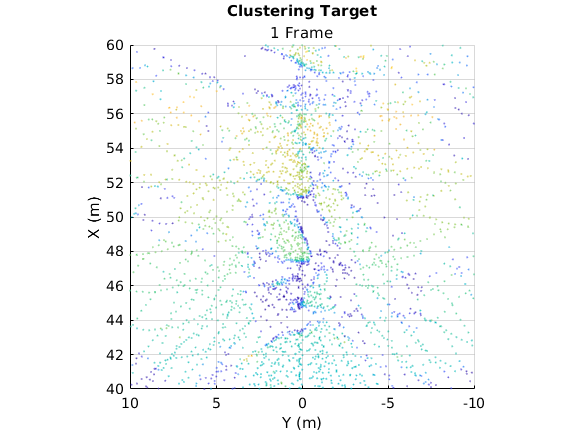
\includegraphics[width=0.95\linewidth]{figs/660frame.png}
  \caption{\textbf{Scene 2, 1 Frame}}
  \label{fig:660Frame}
\end{minipage}%
\begin{minipage}{.5\textwidth}
  \centering
  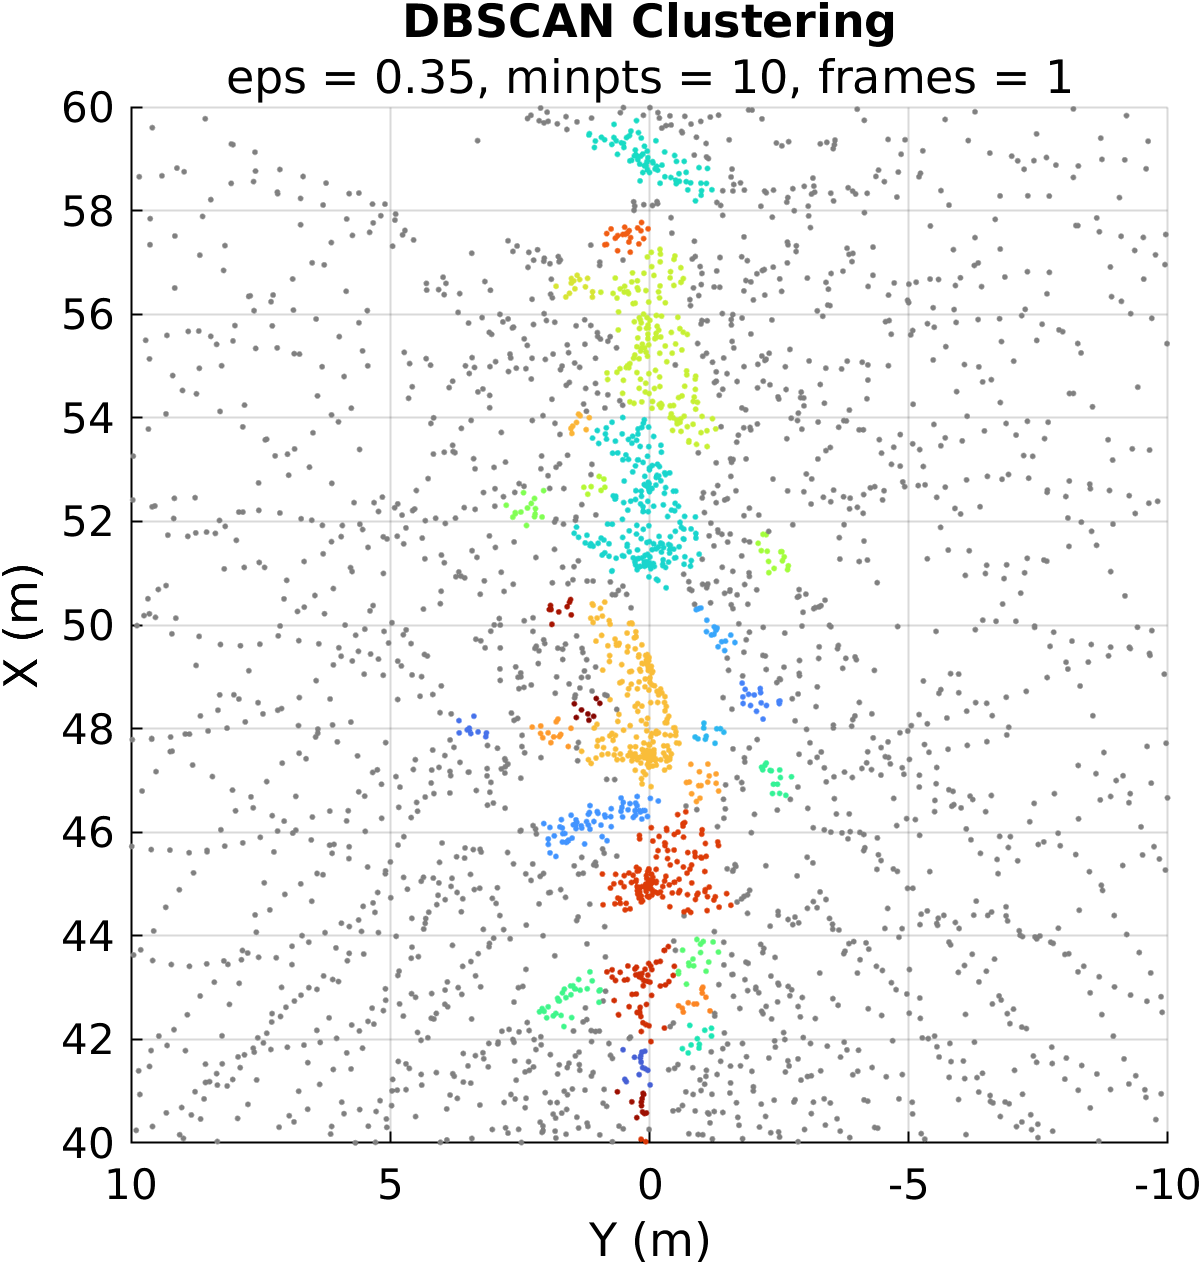
\includegraphics[width=0.95\linewidth]{figs/660_DB.png}
  \caption{\textbf{DBScan}}
  \label{fig:clust660DB}
\end{minipage}
\end{figure}
%----------------------------------------------------

%----------------------------------------------------
\begin{figure}[H]
\centering
\begin{minipage}{.5\textwidth}
  \centering
  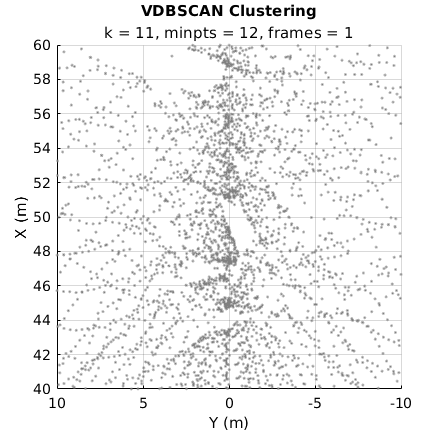
\includegraphics[width=0.95\linewidth]{figs/660_VDB.png}
  \caption{\textbf{VDBScan}}
  \label{fig:clust660VDB}
\end{minipage}%
\begin{minipage}{.5\textwidth}
  \centering
  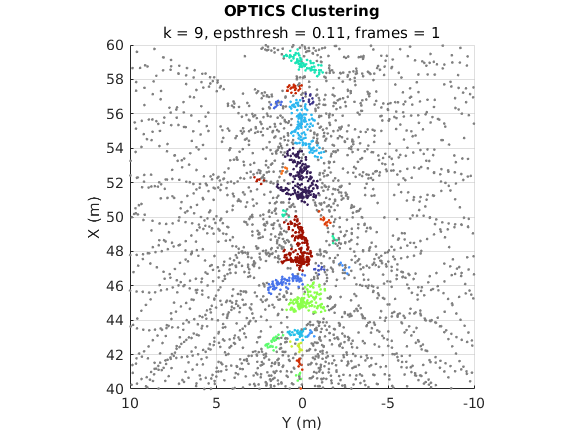
\includegraphics[width=0.95\linewidth]{figs/660_OPT.png}
  \caption{\textbf{OPTICS}}
  \label{fig:clust660OPT}
\end{minipage}
\end{figure}
%----------------------------------------------------

In the single frame target (Figure \ref{fig:660Frame}), \ac{DBScan} and \ac{OPTICS} performed similarly, identifying both clusters A and B with similar shapes and distributions, with \ac{DBScan} assigning slightly more points to each cluster. Both algorithms predominantly identified points on the edges of the pancake floes, with few points assigned to the interior regions of the clusters.

%----------------------------------------------------
\begin{figure}[H]
\centering
\begin{minipage}{.5\textwidth}
  \centering
  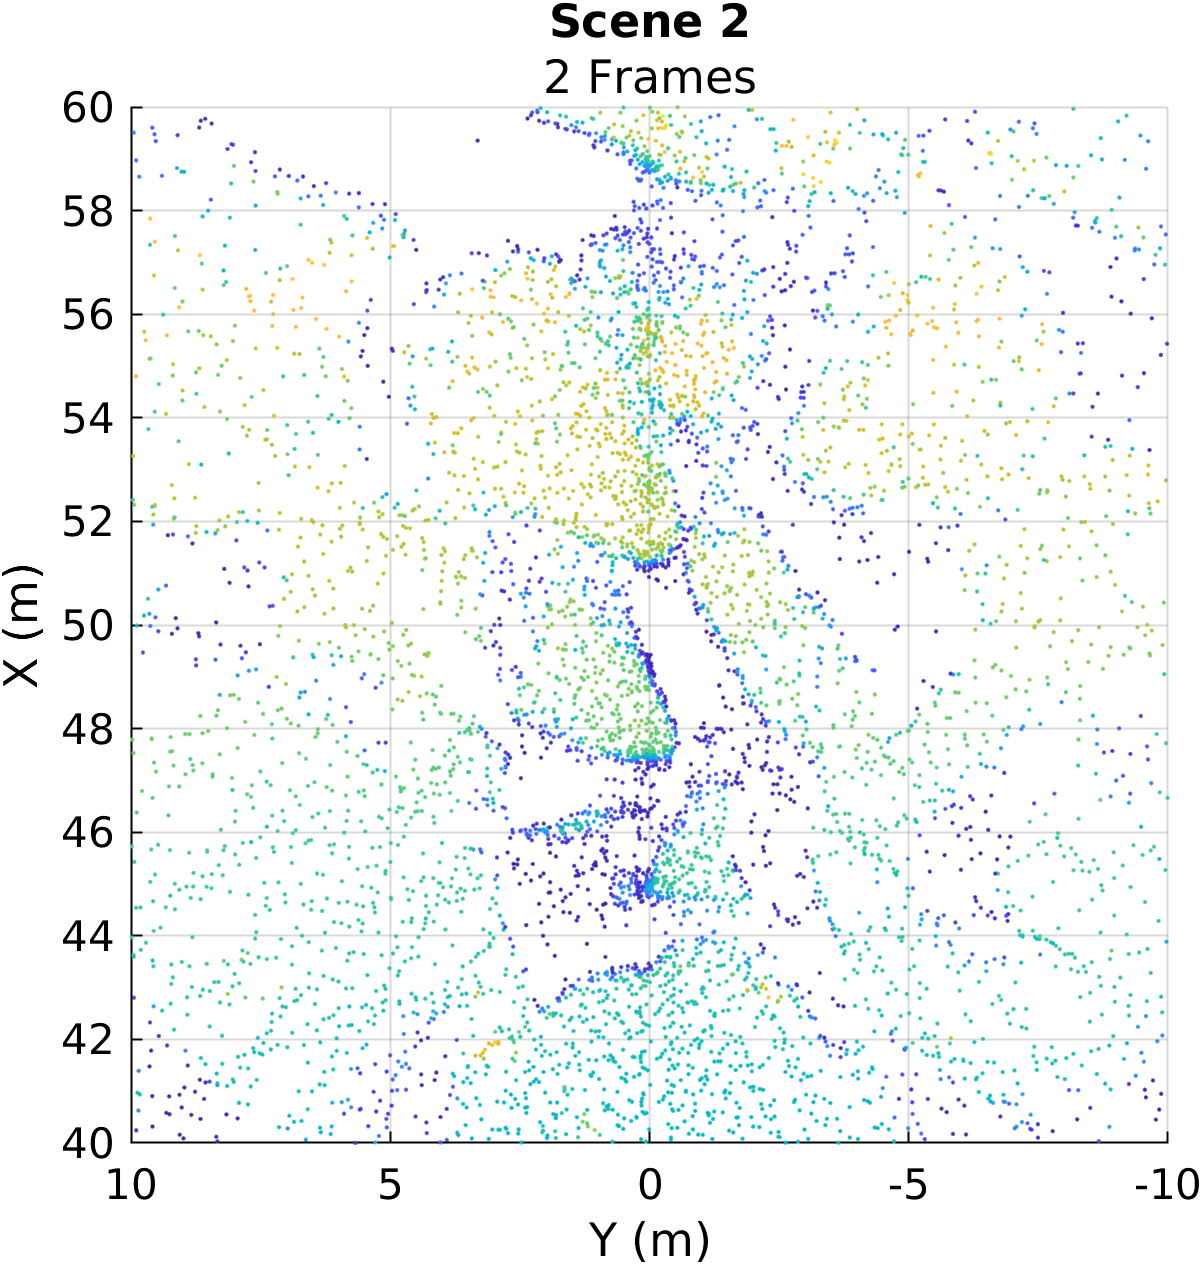
\includegraphics[width=0.95\linewidth]{figs/661frame.png}
  \caption{\textbf{Scene 2, 2 Frames}}
  \label{fig:661Frame}
\end{minipage}%
\begin{minipage}{.5\textwidth}
  \centering
  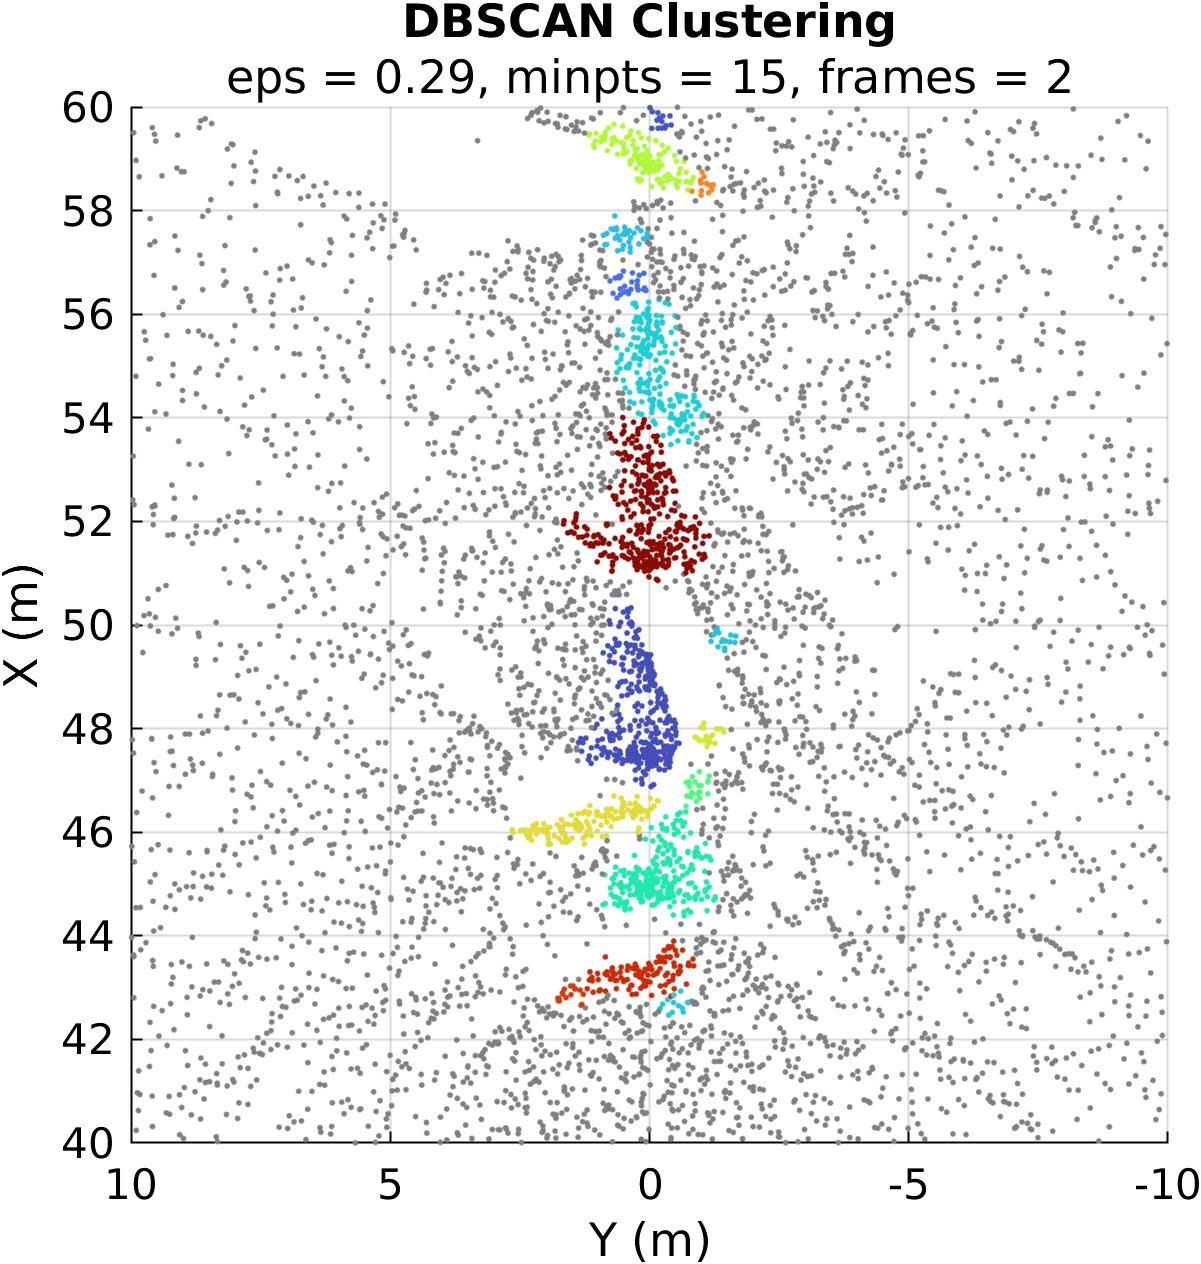
\includegraphics[width=0.95\linewidth]{figs/660_661_DB.png}
  \caption{\textbf{DBScan}}
  \label{fig:clust661DB}
\end{minipage}
\end{figure}
%----------------------------------------------------

%----------------------------------------------------
\begin{figure}[H]
\centering
\begin{minipage}{.5\textwidth}
  \centering
  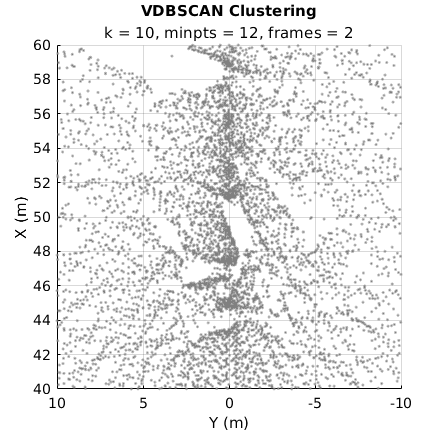
\includegraphics[width=0.95\linewidth]{figs/660_661_VDB.png}
  \caption{\textbf{VDBScan}}
  \label{fig:clust661VDB}
\end{minipage}%
\begin{minipage}{.5\textwidth}
  \centering
  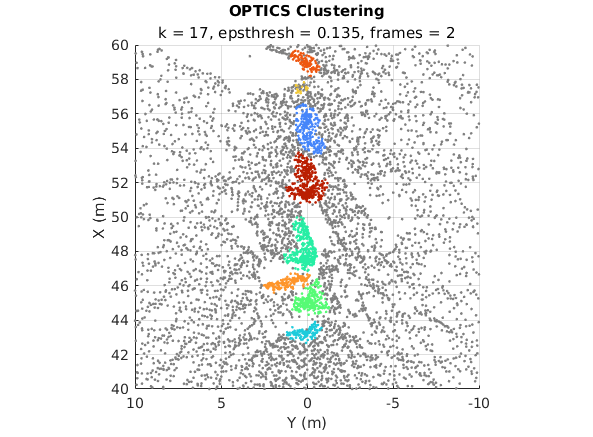
\includegraphics[width=0.95\linewidth]{figs/660_661_OPT.png}
  \caption{\textbf{OPTICS}}
  \label{fig:clust661OPT}
\end{minipage}
\end{figure}
%----------------------------------------------------

In the two frame target (Figure \ref{fig:661Frame}), \ac{DBScan} and \ac{OPTICS} again performed similarly, identifying both clusters A and B with similar shapes and distributions. However, both algorithms assigned points to cluster A, in the region of  x = 51 m, y = -1  m, that are most likely not part of the identified pancake floe, but rather the edge of an adjacent pancake floe as visible in the raw point cloud data, see Figure \ref{fig:661Frame}. Additionally, \ac{OPTICS} assigned more points to cluster B than \ac{DBScan}, predominantly in the interior (left edge of the cluster) of the identified pancake floe.

%----------------------------------------------------
\begin{figure}[H]
    \centering
    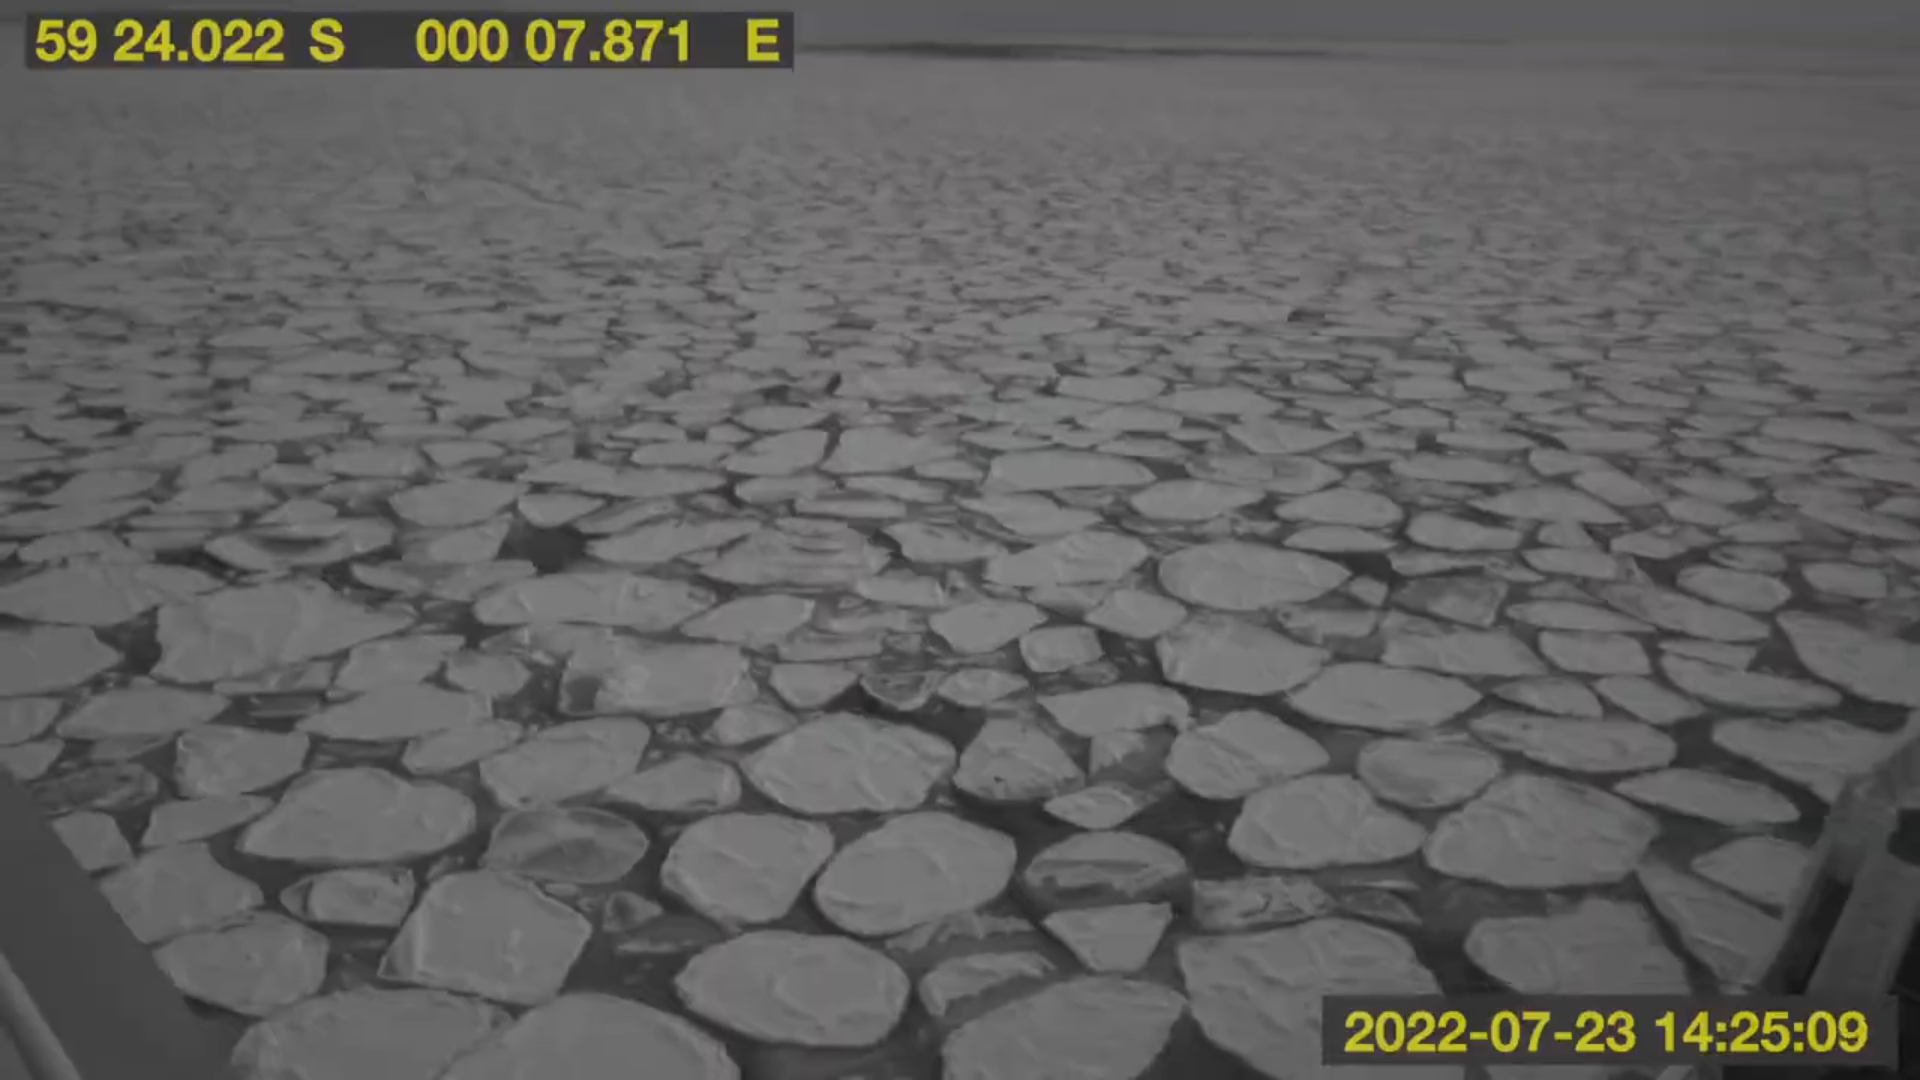
\includegraphics[width=0.8\textwidth]{figs/660cam.PNG}
    \caption{\textbf{Scene 2 Video Still}}
    \label{fig:660}
\end{figure}
%----------------------------------------------------

%----------------------------------------------------
\subsection{Scene 3 - 24 July 2022}
\label{subsec:ch7.section4.subsec3}

Cluster A is the central orange group and cluster B is the lime green group below group A in Figure \ref{fig:clust980DB}. These two clusters were identified by all three algorithms in both single frame and two frame concatenated targets.

%----------------------------------------------------
\begin{table}[H]
\centering
\begin{tabular}{|l|l|r|r|r|}
\hline
\textbf{No Frames} & \textbf{Cluster} & \multicolumn{1}{l|}{\textbf{DBScan}} & \multicolumn{1}{l|}{\textbf{VDBScan}} & \multicolumn{1}{l|}{\textbf{OPTICS}} \\ \hline
\multirow{2}{*}{1} & A                & 198                                  & 189                                   & 189                                  \\ \cline{2-5} 
                   & B                & 147                                  & 125                                   & 153                                  \\ \hline
\multirow{2}{*}{2} & A                & 302                                  & 324                                   & 335                                  \\ \cline{2-5} 
                   & B                & 244                                  & 303                                   & 280                                  \\ \hline
\end{tabular}
\caption{Scene 2 Points per Cluster}
\label{tab:980Clust}
\end{table}
%----------------------------------------------------

%----------------------------------------------------
\begin{figure}[H]
\centering
\begin{minipage}{.5\textwidth}
  \centering
  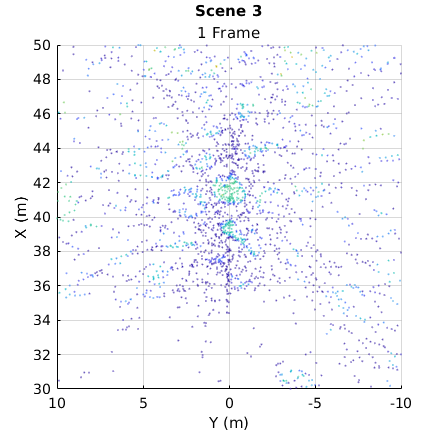
\includegraphics[width=0.95\linewidth]{figs/980frame.png}
  \caption{\textbf{Scene 3, 1 Frame}}
  \label{fig:980Frame}
\end{minipage}%
\begin{minipage}{.5\textwidth}
  \centering
  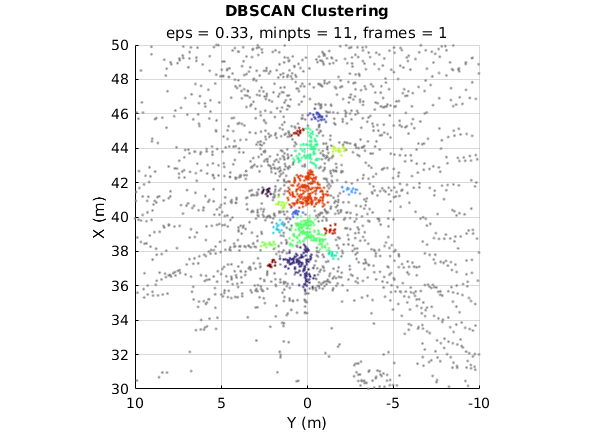
\includegraphics[width=0.95\linewidth]{figs/980_DB.png}
  \caption{\textbf{DBScan}}
  \label{fig:clust980DB}
\end{minipage}
\end{figure}
%----------------------------------------------------

%----------------------------------------------------
\begin{figure}[H]
\centering
\begin{minipage}{.5\textwidth}
  \centering
  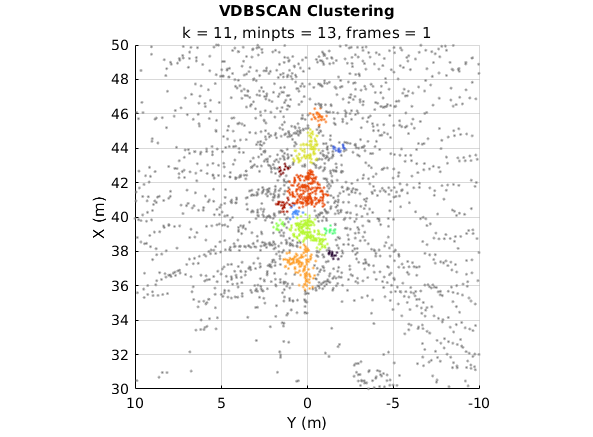
\includegraphics[width=0.95\linewidth]{figs/980_VDB.png}
  \caption{\textbf{VDBScan}}
  \label{fig:clust980VDB}
\end{minipage}%
\begin{minipage}{.5\textwidth}
  \centering
  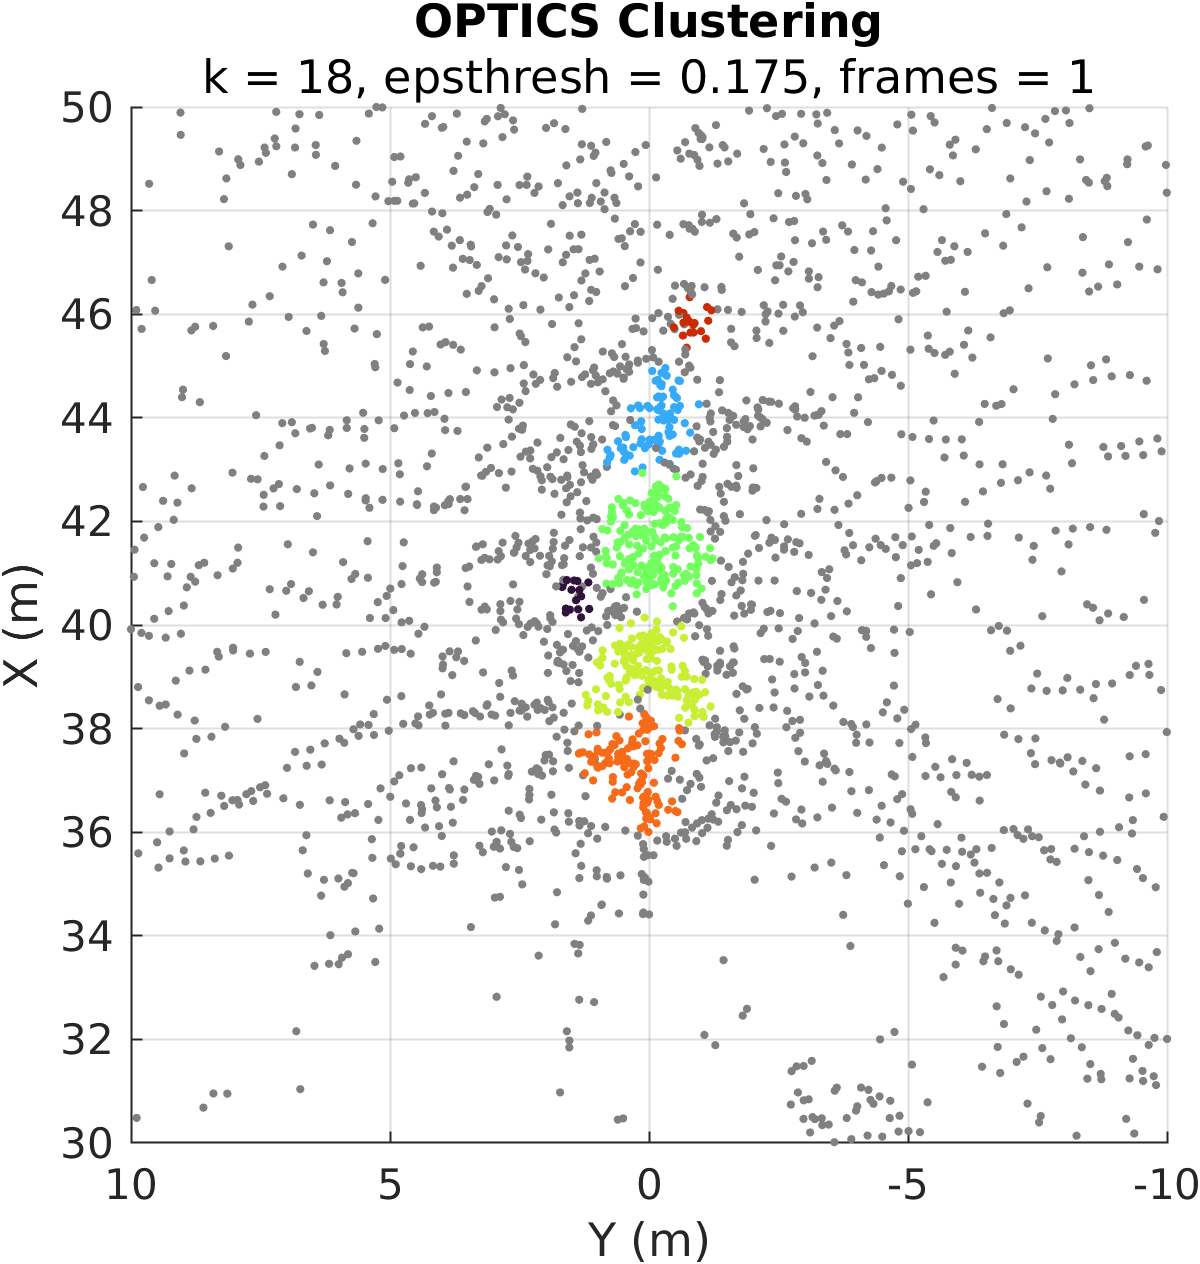
\includegraphics[width=0.95\linewidth]{figs/980_OPT.png}
  \caption{\textbf{OPTICS}}
  \label{fig:clust980OPT}
\end{minipage}
\end{figure}
%----------------------------------------------------

In the single frame target (Figure \ref{fig:980Frame}), all three algorithms performed very similarly in their identification of cluster A, with nearly identical shapes and distributions. The algorithms varied more in their identification of cluster B, with \ac{DBScan} and \ac{OPTICS} producing similar shapes and distributions, including points in the region of x = 39 m, y = 1 m that are likely not part of the identified pancake floe when compared to the raw point cloud data, as seen in Figure \ref{fig:980Frame}. \ac{VDBScan} produced a more compact cluster B, excluding these points.

%----------------------------------------------------
\begin{figure}[H]
\centering
\begin{minipage}{.5\textwidth}
  \centering
  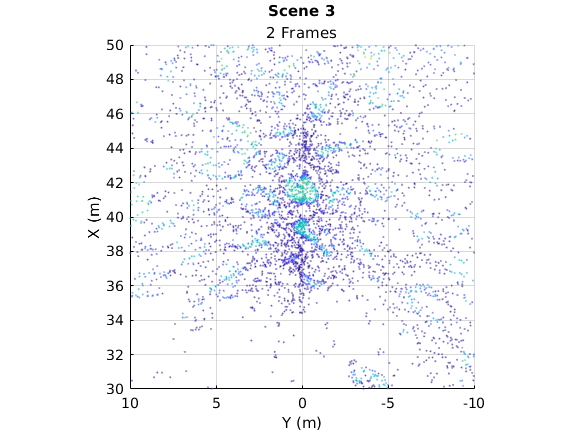
\includegraphics[width=0.95\linewidth]{figs/981frame.png}
  \caption{\textbf{Scene 3, 2 Frames}}
  \label{fig:981Frame}
\end{minipage}%
\begin{minipage}{.5\textwidth}
  \centering
  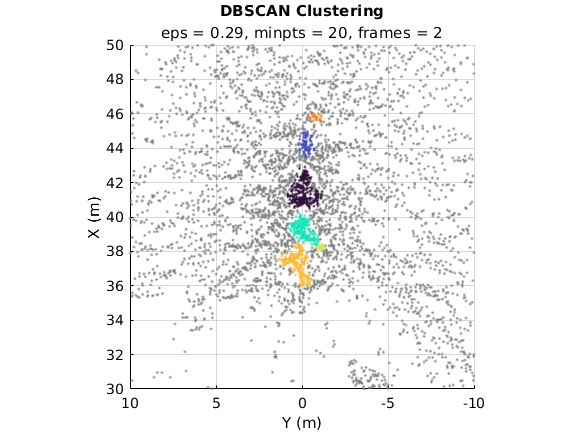
\includegraphics[width=0.95\linewidth]{figs/980_981_DB.png}
  \caption{\textbf{DBScan}}
  \label{fig:clust981DB}
\end{minipage}
\end{figure}
%----------------------------------------------------

%----------------------------------------------------
\begin{figure}[H]
\centering
\begin{minipage}{.5\textwidth}
  \centering
  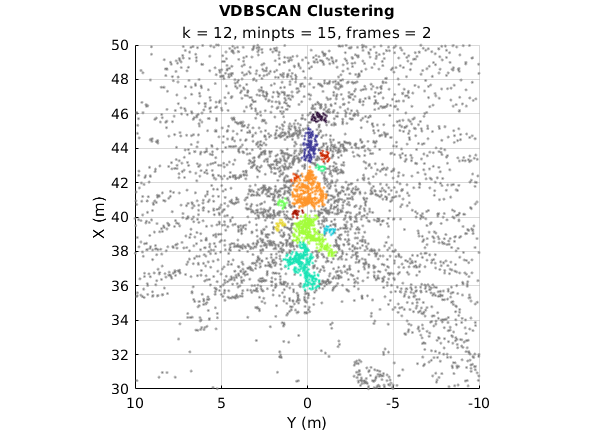
\includegraphics[width=0.95\linewidth]{figs/980_981_VDB.png}
  \caption{\textbf{VDBScan}}
  \label{fig:clust981VDB}
\end{minipage}%
\begin{minipage}{.5\textwidth}
  \centering
  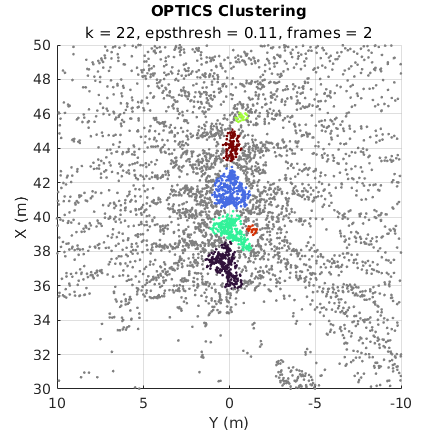
\includegraphics[width=0.95\linewidth]{figs/980_981_OPT.png}
  \caption{\textbf{OPTICS}}
  \label{fig:clust981OPT}
\end{minipage}
\end{figure}
%----------------------------------------------------

In the two frame target (Figure \ref{fig:981Frame}), \ac{DBScan} consistently assigned the least points to both clusters A and B, excluding points that are likely to be part of the identified pancake floes. \ac{VDBScan} and \ac{OPTICS} produced very similar shapes and distributions for cluster A, with \ac{OPTICS} assigning slightly more points. For cluster B, \ac{VDBScan} assigned more points to the edges of the cluster than \ac{OPTICS}, in the regions of x = 38 m, y = -1 m, which are likely part of the identified pancake floe, and x =  39 m, y = 1 m, which are likely not part of the identified pancake floe when compared to the raw point cloud data, see Figure \ref{fig:981Frame}.

%----------------------------------------------------
\begin{figure}[H]
    \centering
    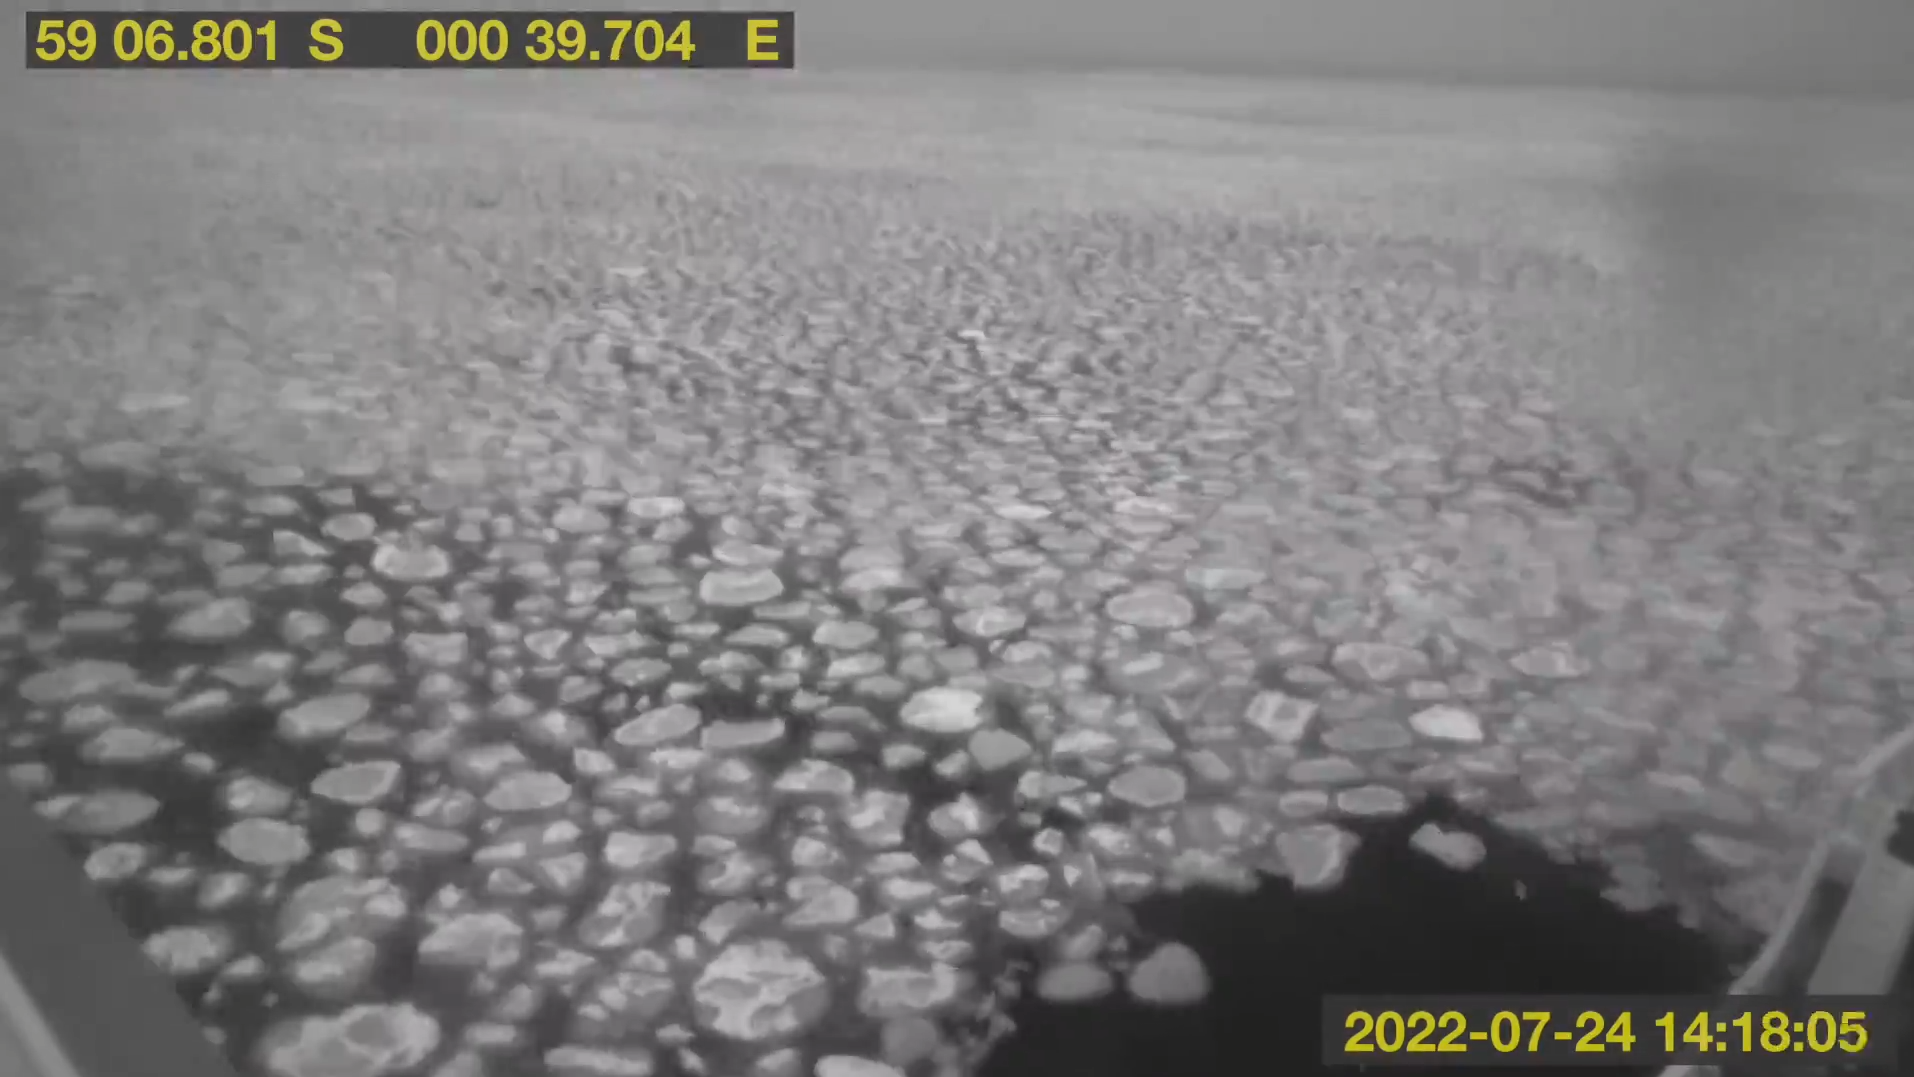
\includegraphics[width=0.8\textwidth]{figs/980cam.PNG}
    \caption{\textbf{Scene 3 Video Still}}
    \label{fig:980}
\end{figure}
%----------------------------------------------------

%----------------------------------------------------
\subsection{Scene 4 - 24 July 2022}
\label{subsec:ch7.section4.subsec4}

Cluster A is the central maroon group and cluster B is the dark blue group below cluster A in Figure \ref{fig:clust5620DB}. These two clusters were identified by all three algorithms in both single frame and two frame concatenated targets. \ac{OPTICS} separated cluster B into two sub-clusters in the single frame target, and all algorithms separated cluster B into multiple sub-clusters in the two frame concatenated target, with \ac{VDBScan} separating it into three sub-clusters.

%----------------------------------------------------
\begin{table}[H]
\centering
\begin{tabular}{|l|l|r|r|r|}
\hline
\textbf{No Frames} & \textbf{Cluster} & \multicolumn{1}{l|}{\textbf{DBScan}} & \multicolumn{1}{l|}{\textbf{VDBScan}} & \multicolumn{1}{l|}{\textbf{OPTICS}} \\ \hline
\multirow{2}{*}{1} & A                & 268                                  & 296                                   & 271                                  \\ \cline{2-5} 
                   & B                & 146                                  & 151                                   & 125 + 22 (147)                       \\ \hline
\multirow{2}{*}{2} & A                & 487                                  & 422                                   & 262                                  \\ \cline{2-5} 
                   & B                & 248 + 49 (297)                       & 195 + 45 + 12 (252)                   & 166 + 22 (188)                        \\ \hline
\end{tabular}
\caption{Scene 4 Points per Cluster}
\label{tab:5620Clust}
\end{table}
%----------------------------------------------------

%----------------------------------------------------
\begin{figure}[H]
\centering
\begin{minipage}{.5\textwidth}
  \centering
  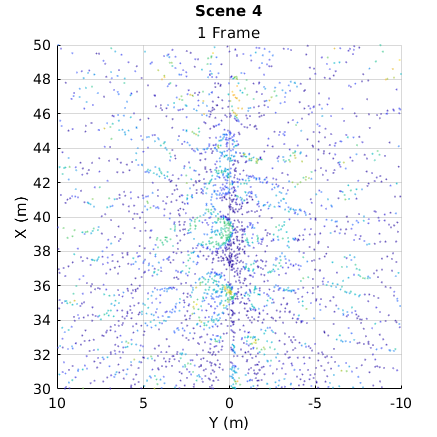
\includegraphics[width=0.95\linewidth]{figs/5620frame.png}
  \caption{\textbf{Scene 4, 1 Frame}}
  \label{fig:5620Frame}
\end{minipage}%
\begin{minipage}{.5\textwidth}
  \centering
  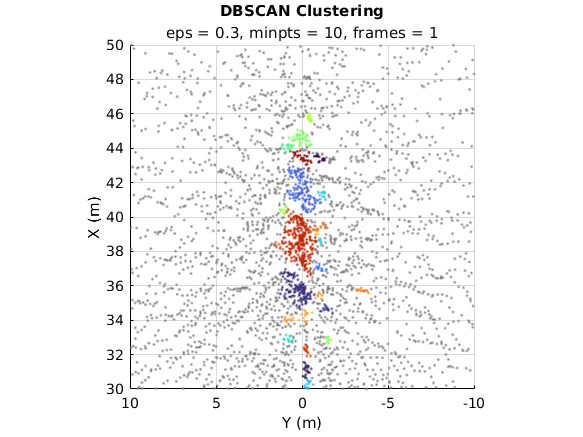
\includegraphics[width=0.95\linewidth]{figs/5620_DB.png}
  \caption{\textbf{DBScan}}
  \label{fig:clust5620DB}
\end{minipage}
\end{figure}
%----------------------------------------------------

%----------------------------------------------------
\begin{figure}[H]
\centering
\begin{minipage}{.5\textwidth}
  \centering
  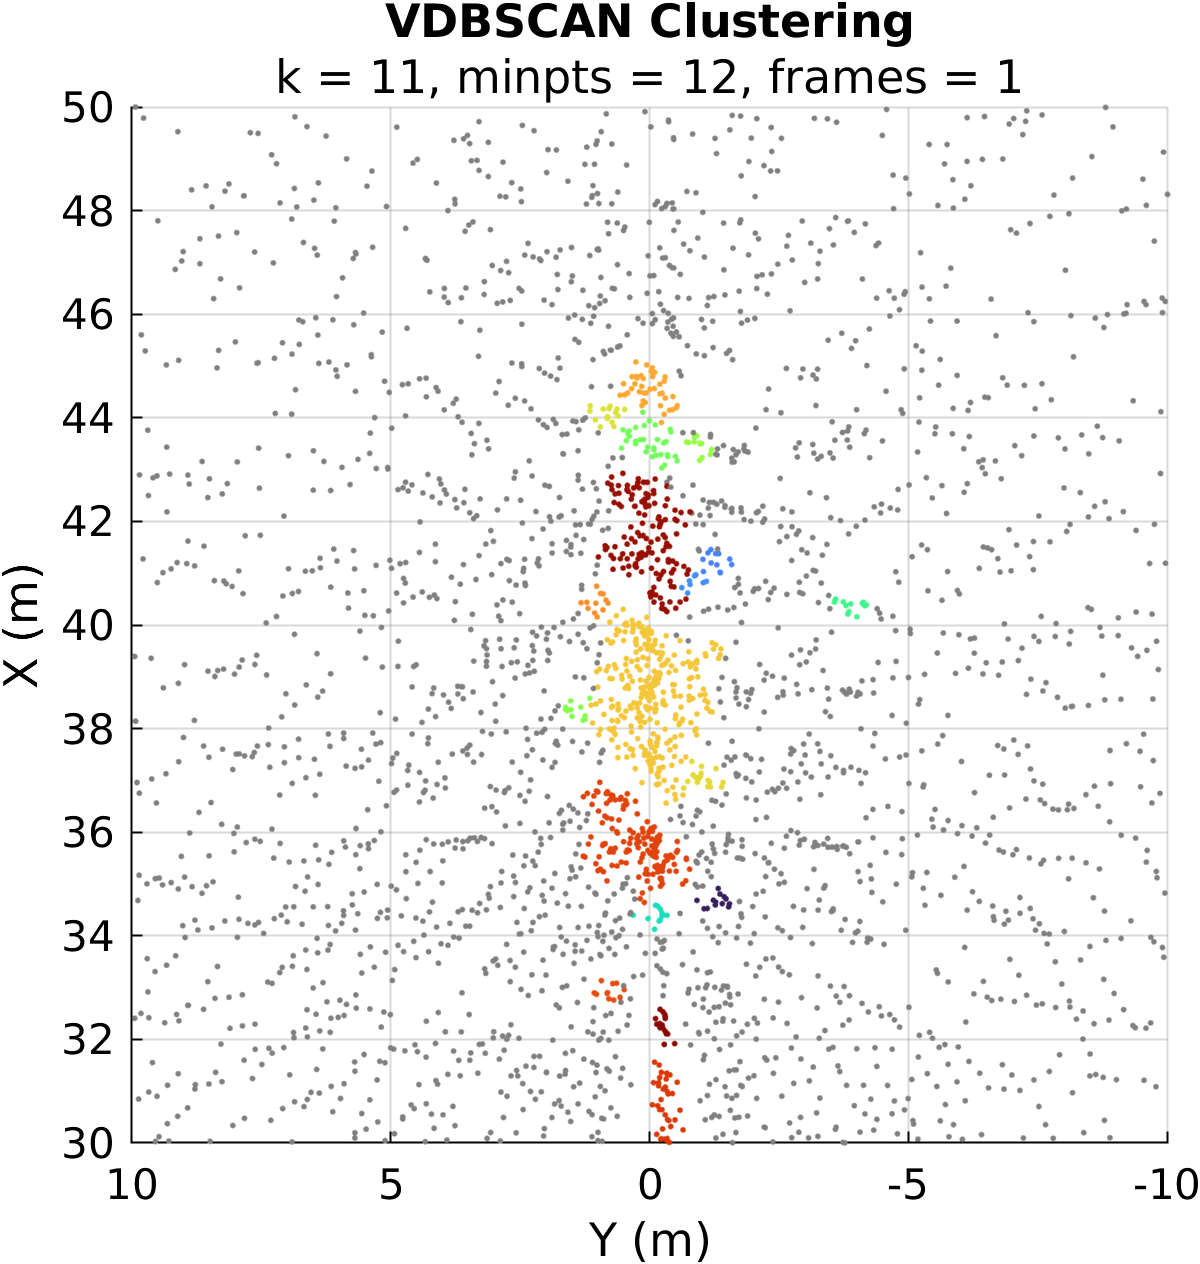
\includegraphics[width=0.95\linewidth]{figs/5620_VDB.png}
  \caption{\textbf{VDBScan}}
  \label{fig:clust5620VDB}
\end{minipage}%
\begin{minipage}{.5\textwidth}
  \centering
  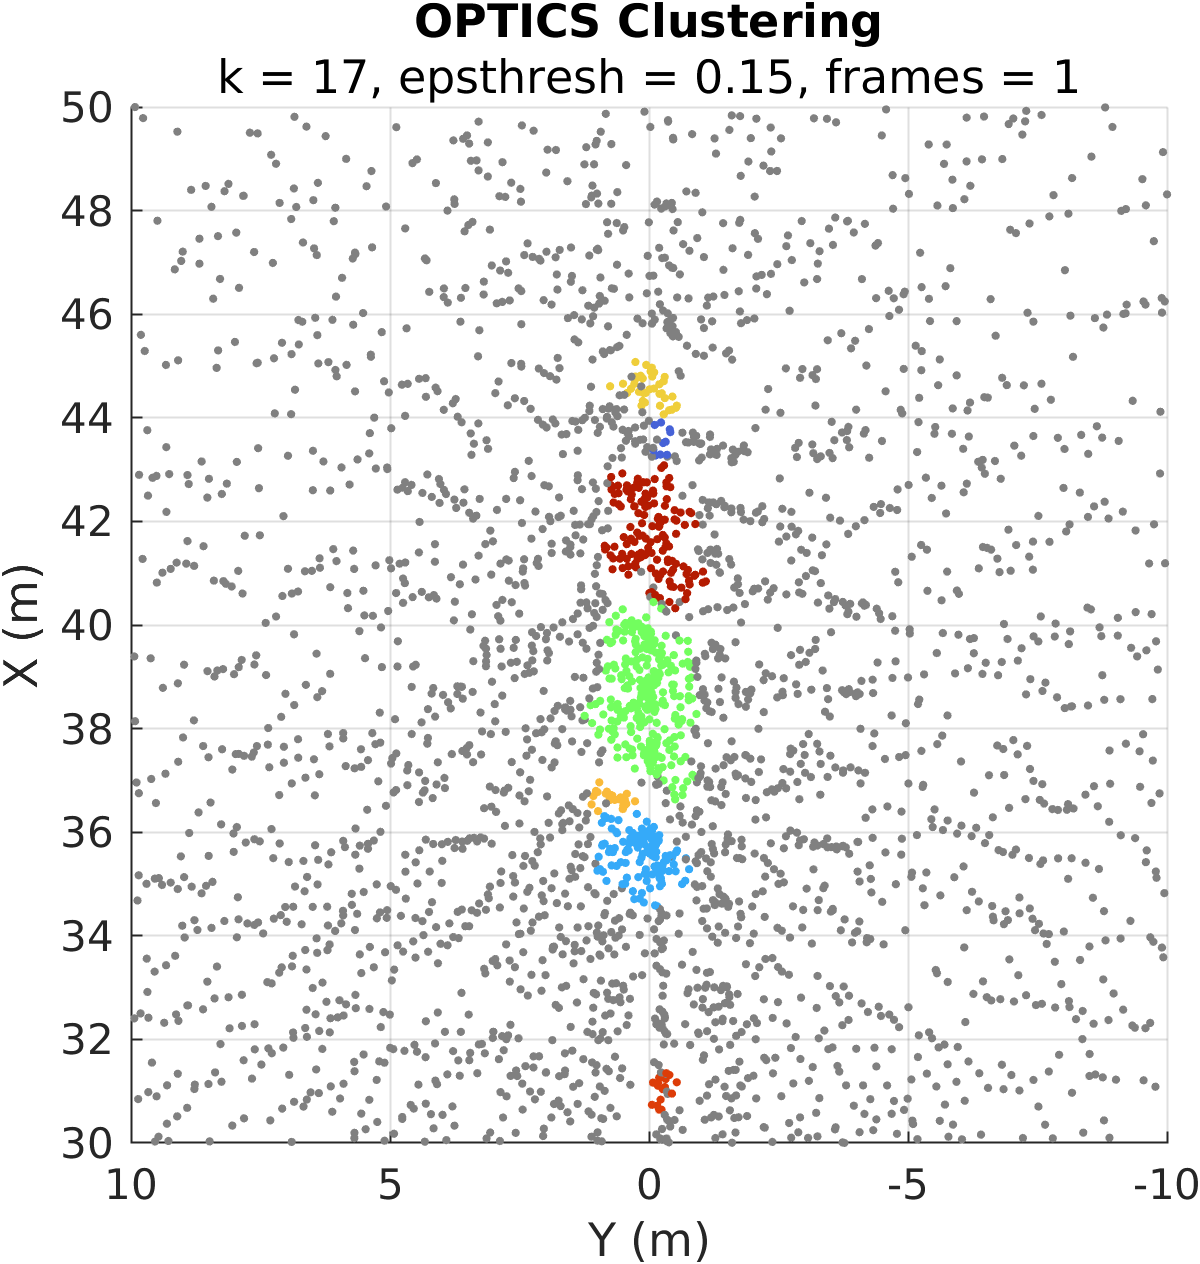
\includegraphics[width=0.95\linewidth]{figs/5620_OPT.png}
  \caption{\textbf{OPTICS}}
  \label{fig:clust5620OPT}
\end{minipage}
\end{figure}
%----------------------------------------------------

In the single frame target (Figure \ref{fig:5620Frame}), all three algorithms performed similarly in their identification of cluster A, with nearly identical shapes and distributions. All algorithms included points in the region of x = 38 m, y = 0 m, that are likely not part of the identified pancake floe, when compared to the raw point cloud data, as seen in Figure \ref{fig:5620Frame}. For cluster B, besides the sub-clustering by \ac{OPTICS}, all algorithms produced similar shapes and distributions. 

%----------------------------------------------------
\begin{figure}[H]
\centering
\begin{minipage}{.5\textwidth}
  \centering
  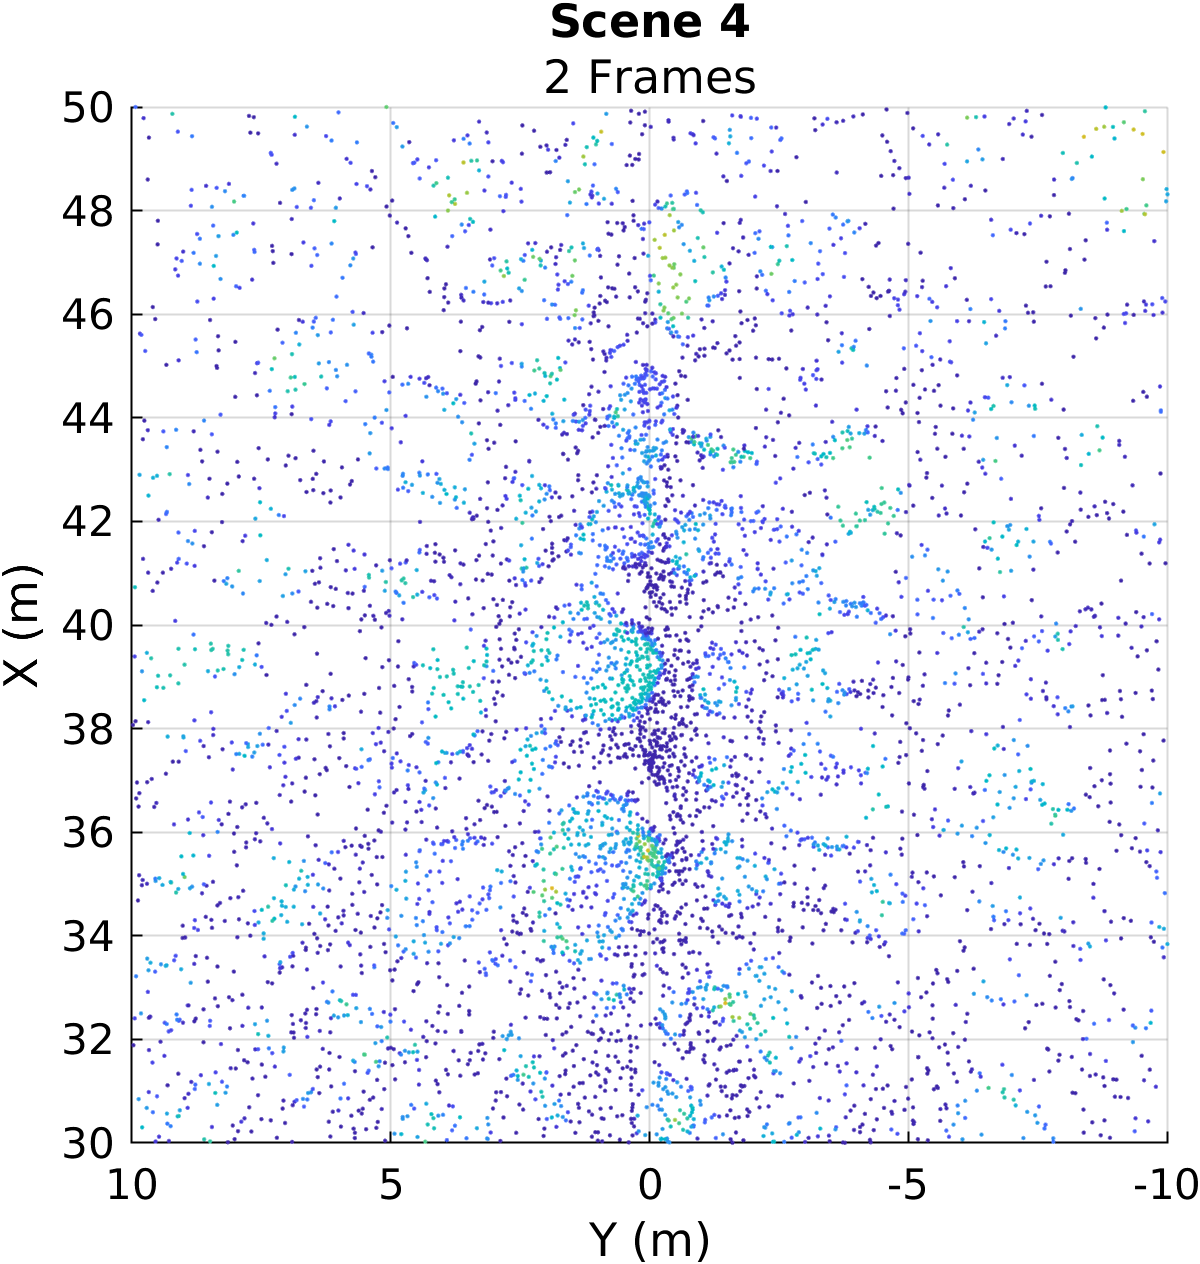
\includegraphics[width=0.95\linewidth]{figs/5621frame.png}
  \caption{\textbf{Scene 4, 2 Frames}}
  \label{fig:5621Frame}
\end{minipage}%
\begin{minipage}{.5\textwidth}
  \centering
  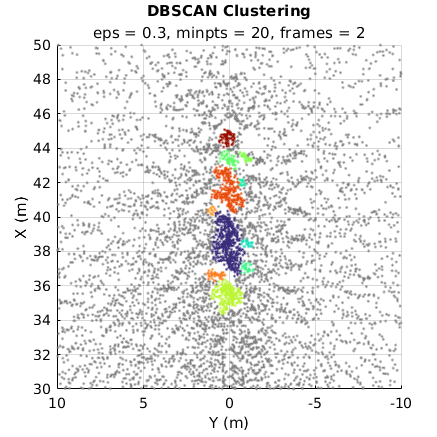
\includegraphics[width=0.95\linewidth]{figs/5620_5621_DB.png}
  \caption{\textbf{DBScan}}
  \label{fig:clust5621DB}
\end{minipage}
\end{figure}
%----------------------------------------------------

%----------------------------------------------------
\begin{figure}[H]
\centering
\begin{minipage}{.5\textwidth}
  \centering
  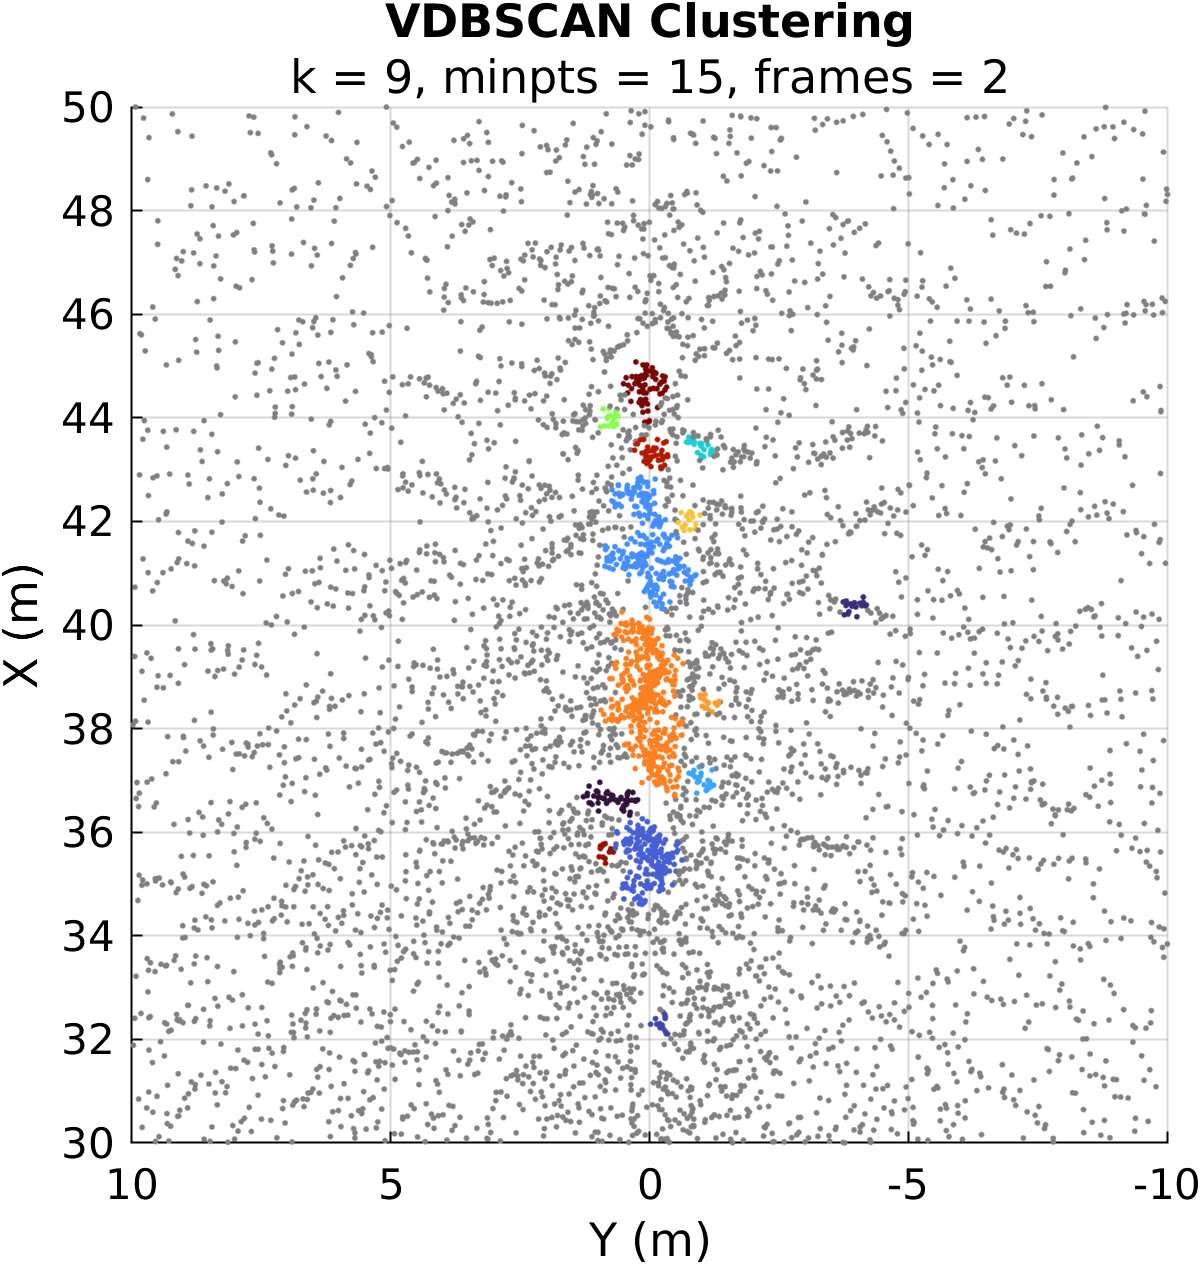
\includegraphics[width=0.95\linewidth]{figs/5620_5621_VDB.png}
  \caption{\textbf{VDBScan}}
  \label{fig:clust5621VDB}
\end{minipage}%
\begin{minipage}{.5\textwidth}
  \centering
  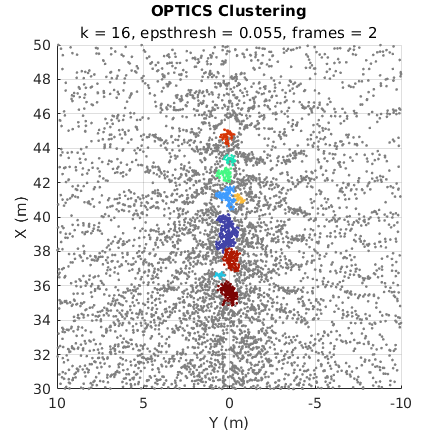
\includegraphics[width=0.95\linewidth]{figs/5620_5621_OPT.png}
  \caption{\textbf{OPTICS}}
  \label{fig:clust5621OPT}
\end{minipage}
\end{figure}
%----------------------------------------------------

In the two frame target (Figure \ref{fig:5621Frame}), \ac{OPTICS} was the only algorithm that excluded points in the region of x = 38 m, y = 0 m. These points are likely not part of the identified pancake floe but rather the edge of an adjacent pancake floe, or a region of frazil ice. This is corroborated by the raw point cloud data, as seen in Figure \ref{fig:5621Frame} and the ice structure seen in the video still, Figure \ref{fig:5620}. For cluster B, \ac{OPTICS} assigned the least points to the cluster, while \ac{DBScan} assigned the most points and \ac{VDBScan} produced a shape and distribution between the other two algorithms. The result produced by \ac{DBScan} is likely the most accurate representation of the pancake floe when compared to the raw point cloud data in Figure \ref{fig:5621Frame}.

%----------------------------------------------------
\begin{figure}[H]
    \centering
    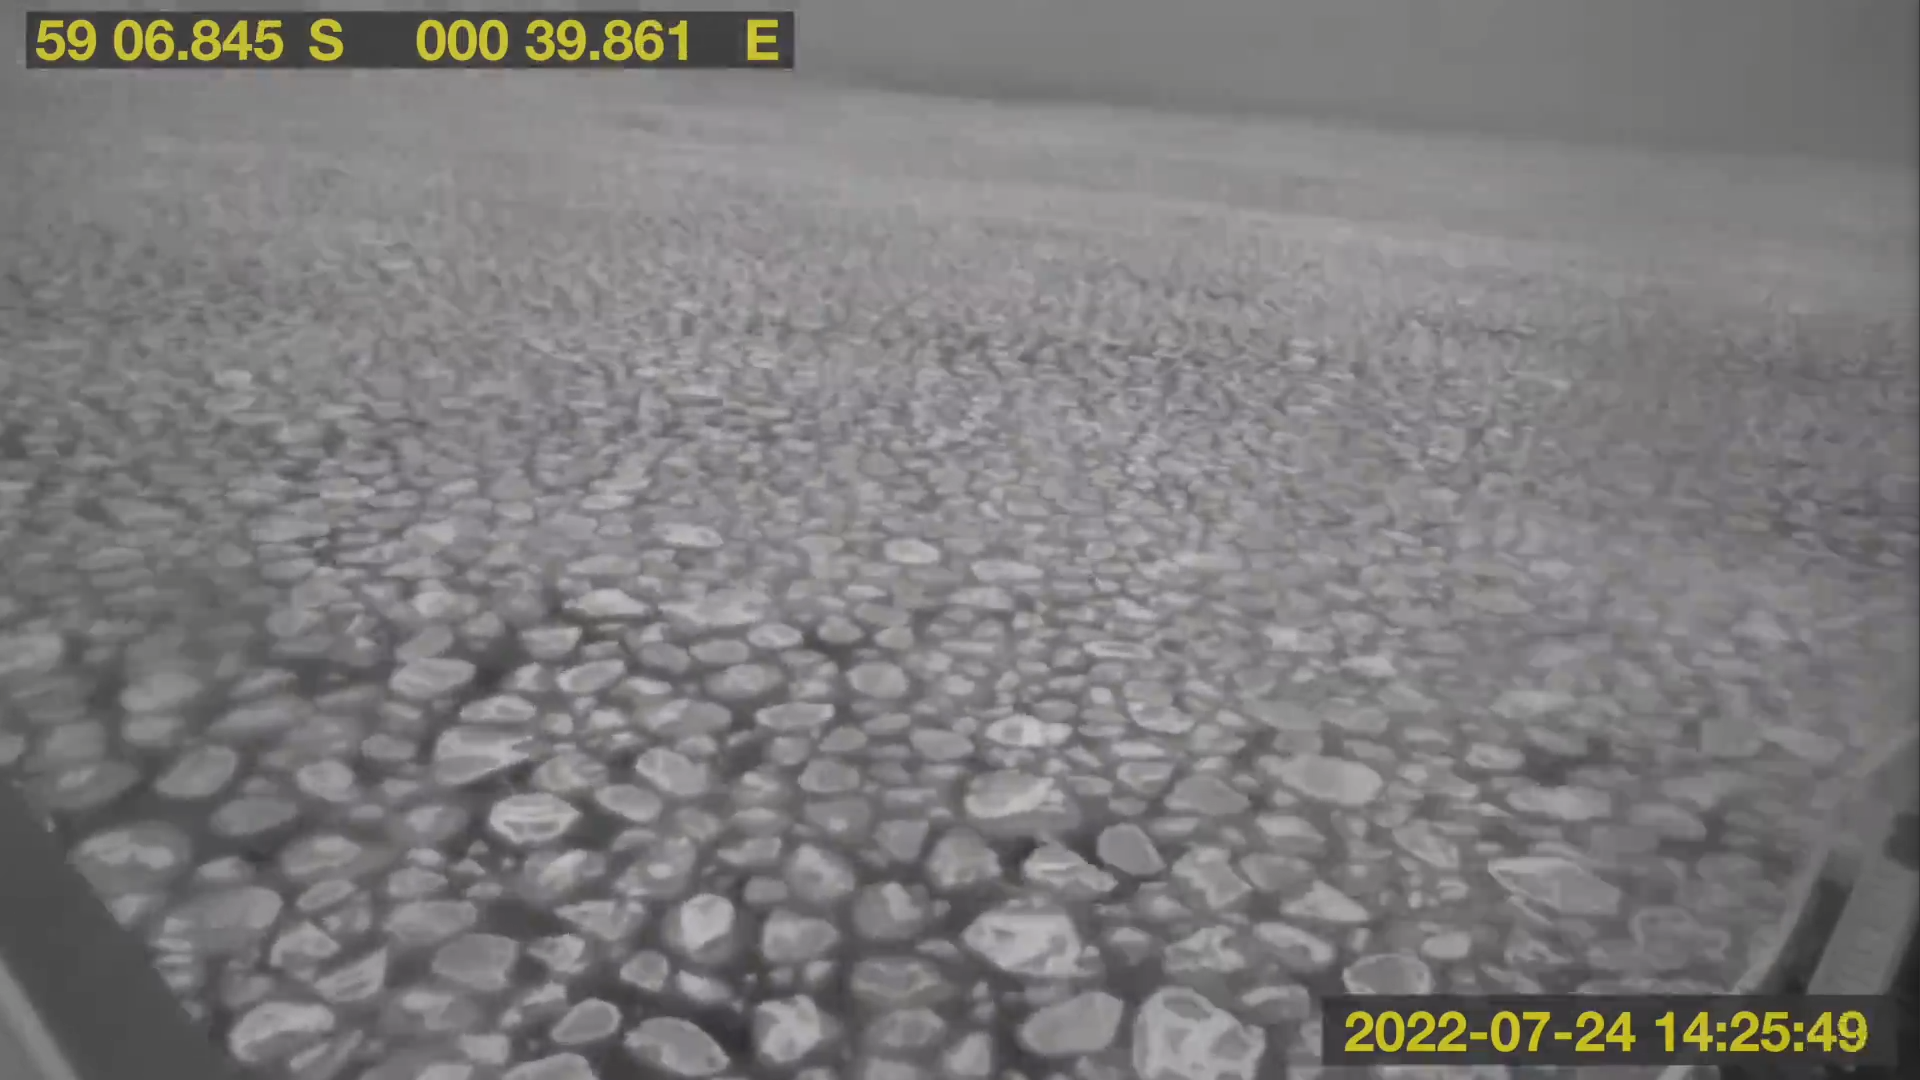
\includegraphics[width=0.8\textwidth]{figs/5620cam.PNG}
    \caption{\textbf{Scene 4 Video Still}}
    \label{fig:5620}
\end{figure}
%----------------------------------------------------

%****************************************************
% END
%****************************************************